\capitulo{3}{Metodología}

\section{Descripción de los datos.}

Para la elaboración del proyecto no se han empleado datos predefinidos obtenidos de bases de datos existentes, se han utilizado datos de elaboración propia. Estos datos se pueden diferenciar entre datos proporcionados por los usuarios y datos proporcionados por el dispositivo.

Por un lado, existen los datos que hayan sido proporcionados por el usuario, al crear su cuenta en la aplicación del dispositivo. Estos datos son datos personales, como su nombre, apellidos, nombre de usuario, correo electrónico, edad o contraseña. Estos datos deberán ser debidamente protegidos según las leyes españolas relativas, para más información consultar \textit{Anexo A}.

Por otro lado, tenemos aquellos datos que se recopilan cada vez que se realiza la monitorización de la postura del usuario, ya se encuentre la persona sentada o de pie. Se realizan mediciones cada medio segundo a través del dispositivo. En cada medición se obtendrán en los 3 ejes (ejes \textit{x},\textit{y} y \textit{z}) aceleraciones en $m/s^{2}$, rotaciones en $deg/s$ y ángulos de inclinación en $deg$. Los ángulos de inclinación se han obtenido a partir de la triangulación de las aceleraciones y son los que se han empleado principalmente en el prototipo para la diferenciación entre una buena y una mala postura en base al umbral establecido. La acumulación de estos datos permitirá realizar distintas estadísticas que servirán al usuario para conocer su situación y su evolución al emplear el dispositivo.

Si se detecta una postura perjudicial, porque se ha superado el ángulo umbral durante un tiempo determinado se realizará una señal de biofeedback para que el usuario recupere una postura correcta y de esta forma se logrará que se desarrolle la postura natural correcta y saludable. Una postura correcta prevendrá al usuario de posibles lesiones y permitirá un mejor desarrollo de algunas actividades.

En el futuro, la recopilación de esta serie de datos de gran cantidad de personas puede abrir camino a la realización de estudios estadísticos acerca de la postura en distintas condiciones, como la postura en función de la edad, sexo o actividad.

 
\section{Técnicas y herramientas.}
En este apartado se realiza una recopilación de técnicas y herramientas empleadas o valoradas en el desarrollo del proyecto.

\subsection{Leguajes de programación y bibliotecas empleadas}
En el grado se han enseñado varios lenguajes de programación, como Java, Python, LaTex, R, C++ o Markdown. Durante el desarrollo del proyecto se han empleado algunos de estos lenguajes de programación. Por ejemplo, para la creación de los documentos oficiales se ha empleado el lenguaje LaTex, para la creación de los programas que se incluirán en la placa de Arduino del prototipo se ha empleado C++, mientras que para la presentación del repositorio de GitHub se ha empleado Markdown.

Se han empleado 3 bibliotecas de Arduino que se complementan y facilitan el trabajo con el sensor MPU6050, sensor empleado en la segunda versión del prototipo. Se han empleado la biblioteca estándar de Arduino que permite la comunicación con dispositivos por bus I2C\footnote{\textbf{Bus I2C}: Inter-Integrated Circuit, es el estándar de comunicación entre dispositivos, se basa en el uso de 2 cables, uno como señal de reloj y el otro para el envío de datos. Se trata de una comunicación algo más compleja que el bus SPI.}\cite{I2C} Wire.h\cite{LibWire}, la biblioteca I2Cdev.h\cite{LibI2Cdev} que simplifica el código de comunicación por bus I2C y minimiza el uso de memoria y la biblioteca MPU6050.h\cite{LibMPU6050} que tiene definidos varios métodos y atributos que simplifican el uso de sensores de este tipo pudiendo trabajar de forma simple con los valores registrados del giroscopio y del acelerómetro integrados.


\subsection{Entornos y aplicaciones empleadas.}
Para el desarrollo del proyecto se han empleado una serie de aplicaciones gratuitas que hemos podido conocer y utilizar a lo largo de la realización del grado. 
\begin{itemize}
\item \textbf{Overleaf}\cite{Overleaf}: es un editor LaTeX colaborativo en línea, que se emplea para la creación, edición y publicación de documentos científicos. LaTeX es una herramienta que a partir del procesamiento de un documento de texto plano compuesto por texto y comandos LaTeX por el software de TeX engine convierte los comandos LaTeX y el texto del documento en un archivo PDF profesional. Esta es la herramienta que se ha empleado para la realización de este documento. Se puede acceder a través de https://www.overleaf.com  %(Referencia: https://www.overleaf.com/learn/latex/Learn_LaTeX_in_30_minutes#What_is_LaTeX )

\item \textbf{Diagrams.net}\cite{Diagrams.net}: es una aplicación de código abierto para la realización de diagramas online, con gran cantidad de librerías de formas para su realización. Esta aplicación es la que se ha empleado para la realización de la gran mayoría de diagramas del proyecto y los prototipos de interfaz, para ver los diagramas realizados con esta herramienta se recomienda consultar el \textit{Anexo F}. Se puede acceder a través de: https://www.diagrams.net % Referencia: https://www.diagrams.net/doc/getting-started-editor  

\item \textbf{Tinkercad}\cite{Tinkercad}:es una aplicación web gratuita que permite desarrollar habilidades de diseño 3D, electrónica y programación, sin necesidad de utilizar ningún tipo de software adicional. En este proyecto se ha empleado esta herramienta para la simulación del diseño del circuito electrónico, ya que permite realizar circuitos y componentes desde 0 o empleando sus circuitos predefinidos. Además, esta aplicación consta de un editor de código que permite programar las simulaciones. Se puede acceder a través de: https://www.tinkercad.com %Referencia: https://www.tinkercad.com/circuits 

\item \textbf{Arduino}\cite{Arduino1, Arduino2}: plataforma de código abierto de electrónica basada en hardware y software simple y accesible, originalmente creada para la creación rápida de prototipos. Existen diferentes placas de Arduino con distintas funciones. Se puede introducir en el microcontrolador un conjunto de instrucciones que se quiere que realice el dispositivo mediante el uso del software de Arduino (IDE), estas instrucciones están escritas en el lenguaje de programación Arduino, que es similar a C++ pero simplificado, además se puede expandir el lenguaje utilizando distintas bibliotecas C++. Esta plataforma es muy utilizada y ha permitido crear gran variedad de proyectos. Su sencillez, accesibilidad y coste es lo que ha predispuesto este sistema para realizar el prototipo de este proyecto basado en esta plataforma. 

\item \textbf{GitHub}\cite{GitHub}: plataforma gratuita en línea de código abierto cuyo objetivo principal es el desarrollo colaborativo de software, para ello se basa en su sistema de control de versiones. GitHub fue construida empleando herramientas de código abierto cómo  Ruby on Rails, Go, Primer, React o Kafka. Además, esta plataforma permite no solo la creación de proyectos públicos sino que también proyectos privados, que se guardan en la nube. Por otro lado, GitHub también tiene distintas herramientas que mejoran y dinamizan el desarrollo de los proyectos. Esta plataforma se ha empleado para llevar el seguimiento del proyecto y recopilar todos los documentos relacionados en un repositorio.

\item \textbf{Trello}\cite{Trello}: herramienta gratuita que ayuda a equipos en gestión de proyectos y flujos de trabajo. Esta plataforma tiene varias herramientas para mejorar el flujo de trabajo, como checklists o tarjetas. Esta plataforma es una herramienta alternativa a ZenHub de GitHub y se ha empleado en el proyecto para comunicaciones con el tutor, revisión de documentos iniciales y recopilación de posibles ideas. Se puede acceder a través de: https://trello.com

\end{itemize}

\subsection{Herramientas.}
A continuación tenemos una lista con componentes empleados en el desarrollo de los prototipos.

\begin{itemize}
\item \textbf{Placa de Arduino}\cite{Arduino1,Arduino2}: se utilizará como microcontrolador la placa de Arduino UNO R3. Esta placa es la más sencilla, robusta y utilizada que ofrece Arduino. El microcontrolador basado en ATmega328P\cite{atmega328P}. La placa tiene 14 pines digitales y 6 pines analógicos.Además, cuenta con un conector USB, un conector de alimentación, un botón de reinicio, un resonador de cerámica de 16 MHz y cabezal ICSP.  En la \textit{Figura \ref{fig:arduino}} se puede ver una imagen de la placa componente.
% Referencia: https://www.arduino.cc/en/Guide/Introduction
% Imagen de la placa de arduino UNO
\begin{figure}[h!]
    \centering
    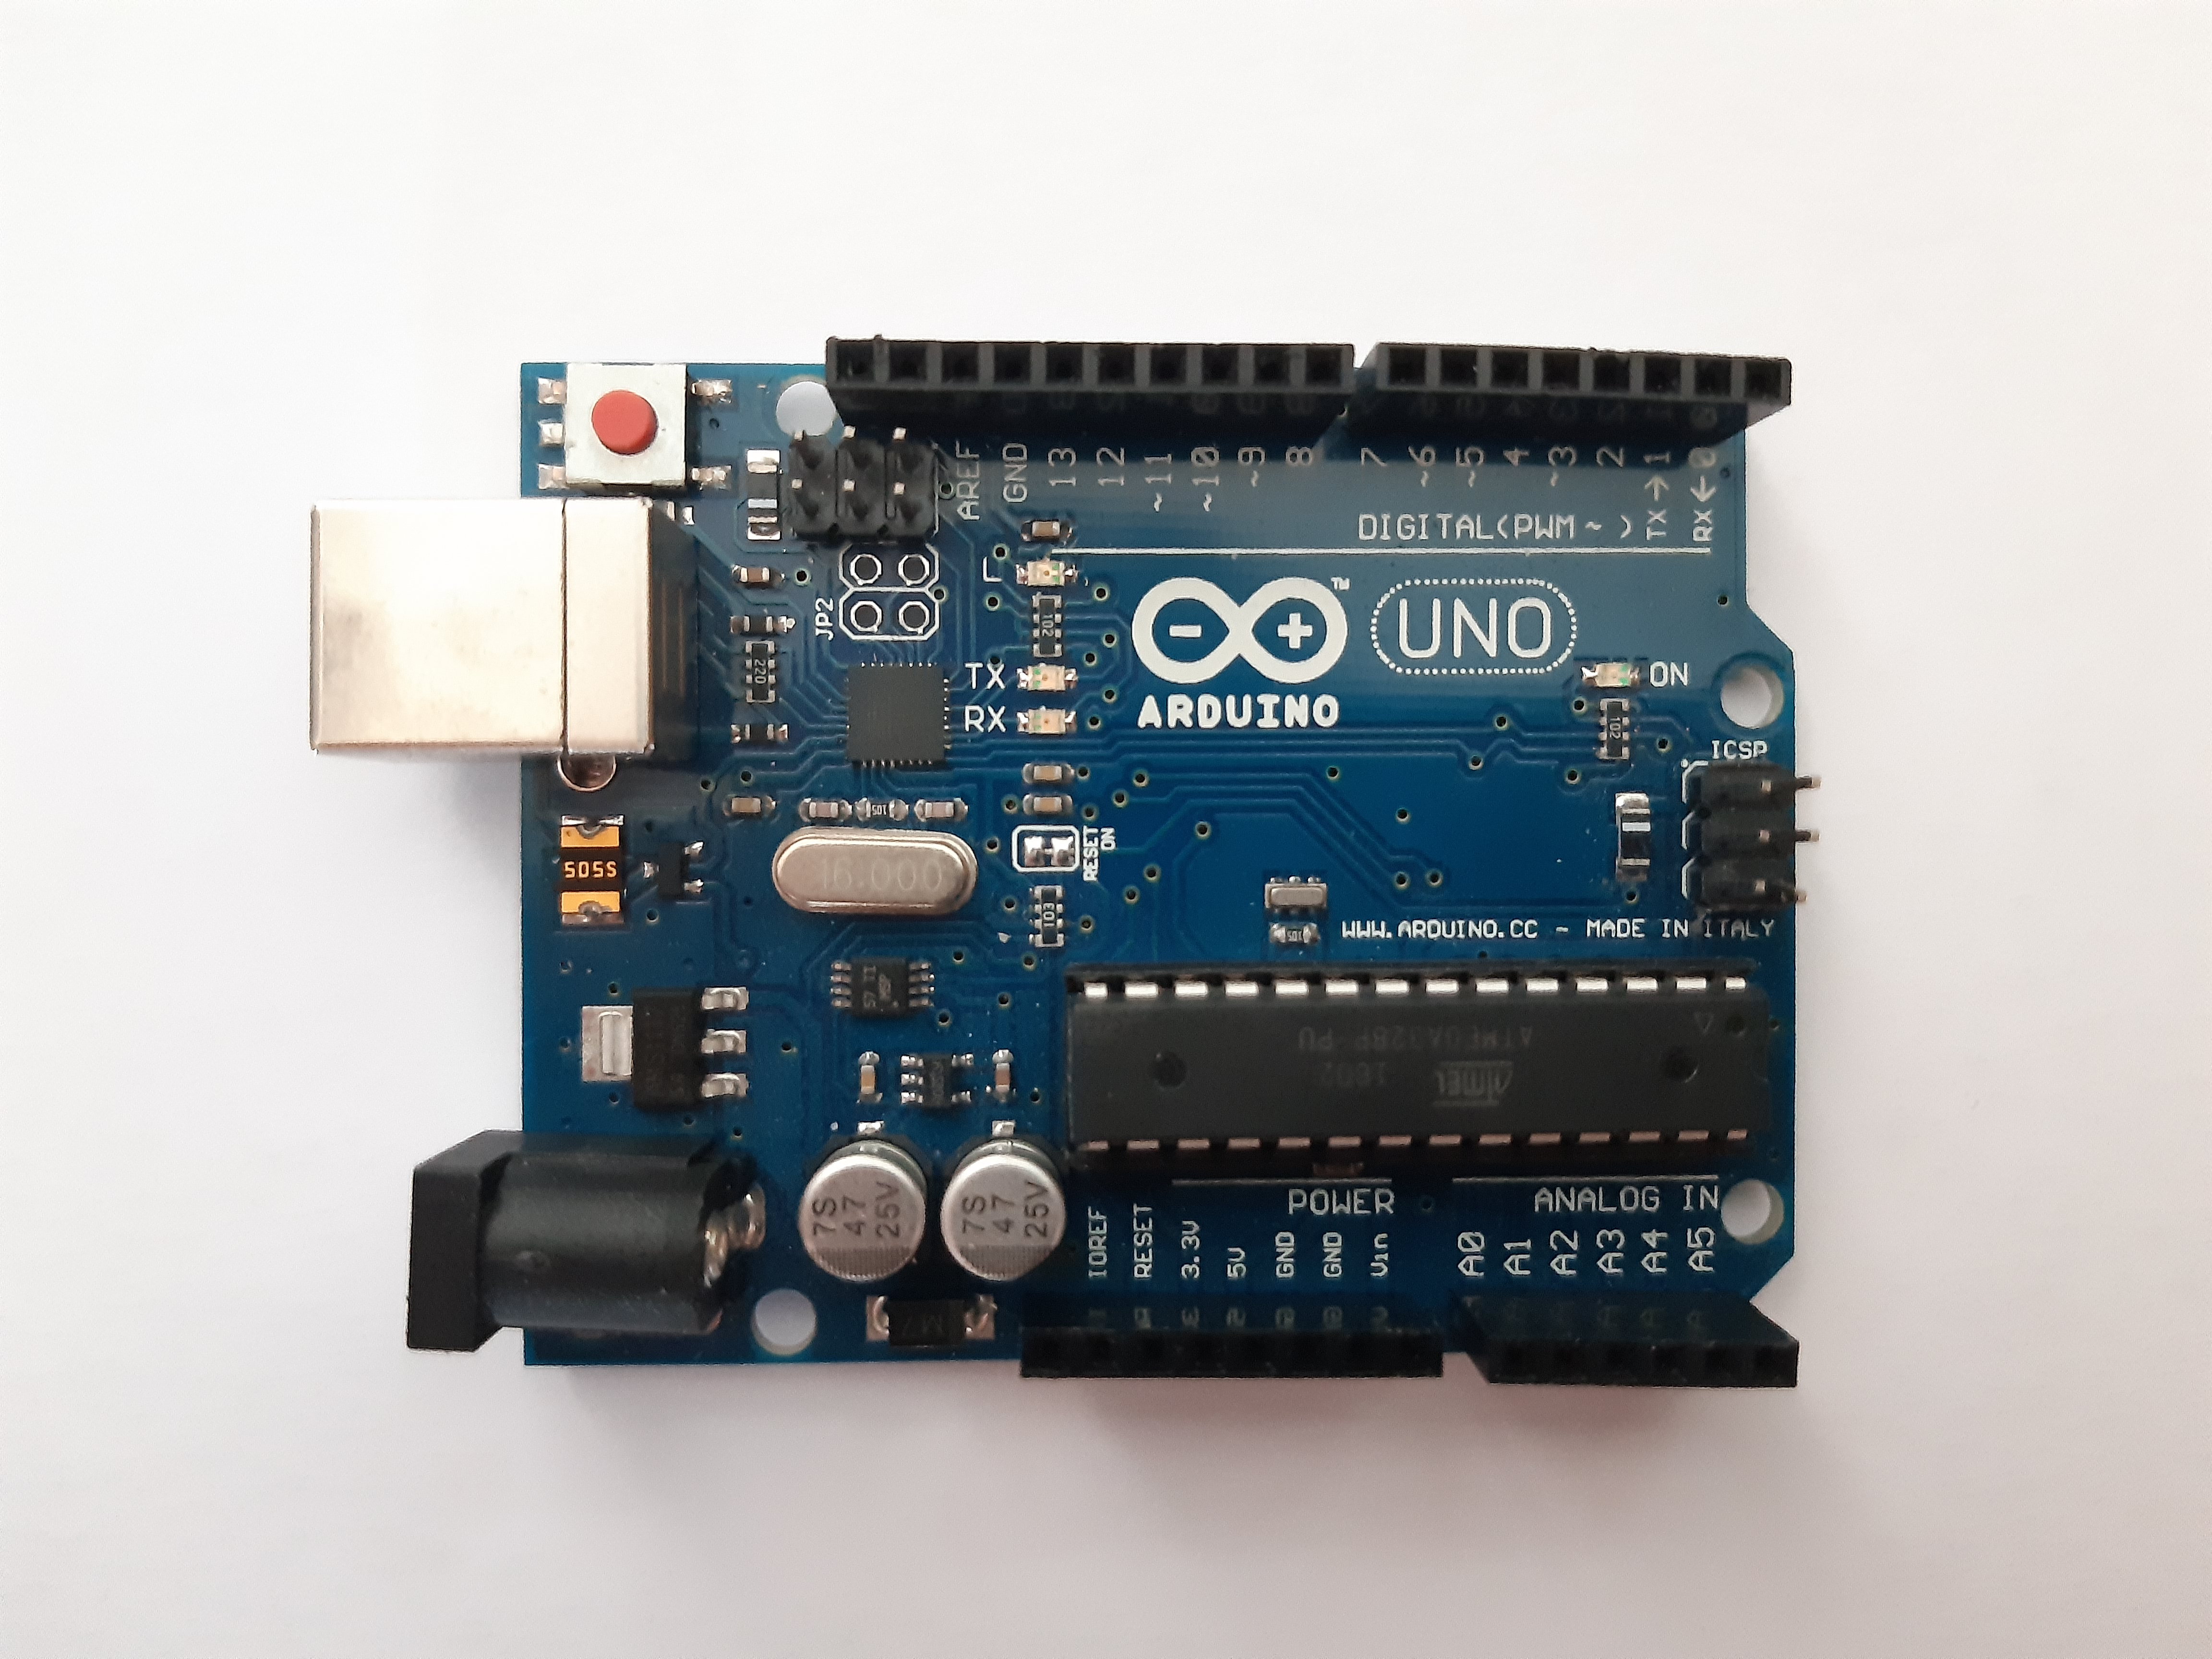
\includegraphics[width=0.5\textwidth]{img/imgArduinoUNO.jpg}
    \caption{Placa de Arduino UNO. Fuente Propia.}
    \label{fig:arduino} 
\end{figure}

\item \textbf{ProtoBoard}: placa sobre la que se construyen los circuitos electrónicos, se trata de una matriz de clavijas donde se insertan los componentes electrónicos. En la \textit{Figura \ref{fig:protoboard}} se puede ver una imagen del componente.
% Imagen de la protoboard.
\begin{figure}[h!]
    \centering
    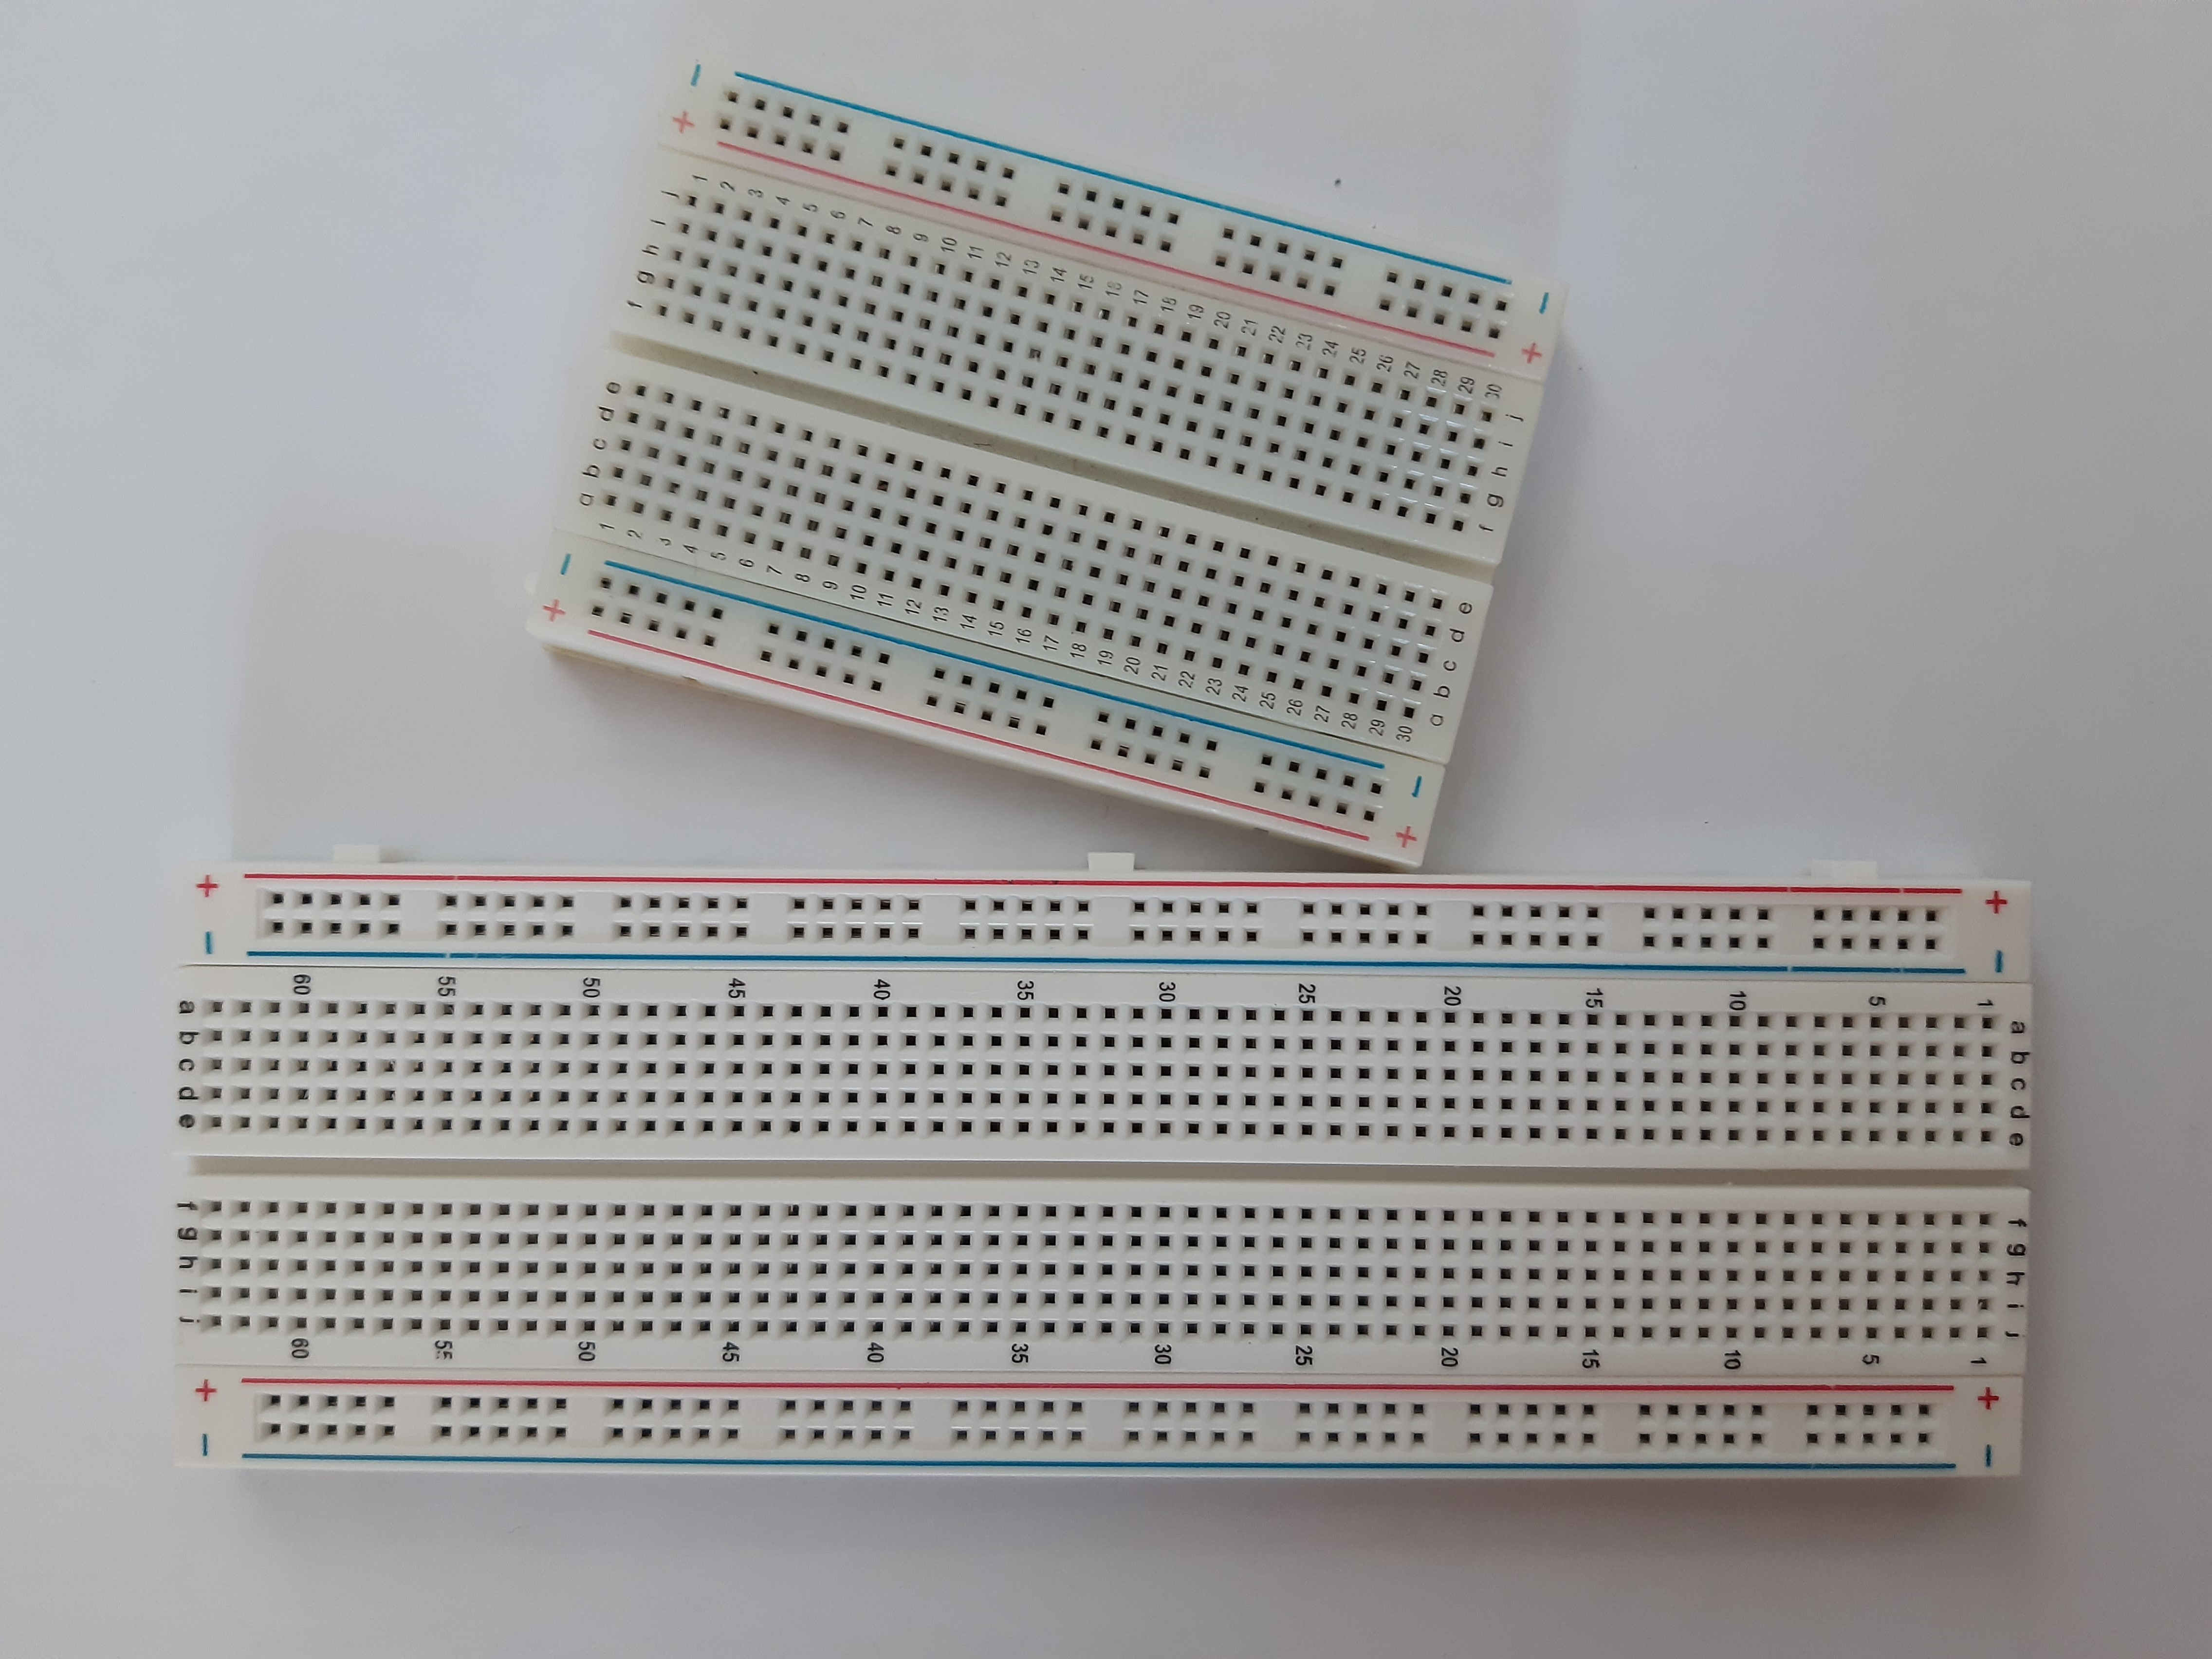
\includegraphics[width=0.5\textwidth]{img/imgProtoboards.JPG}
    \caption{Protoboard. Fuente Propia.}
    \label{fig:protoboard} 
\end{figure}

\item \textbf{Cableado}: alambres de un material conductor cubiertos por un material aislante que permiten las distintas conexiones del circuito. En la \textit{Figura \ref{fig:cableado}} se puede ver una imagen del componente.
% Imagen del los cables que se usarán
\begin{figure}[h!]
    \centering
    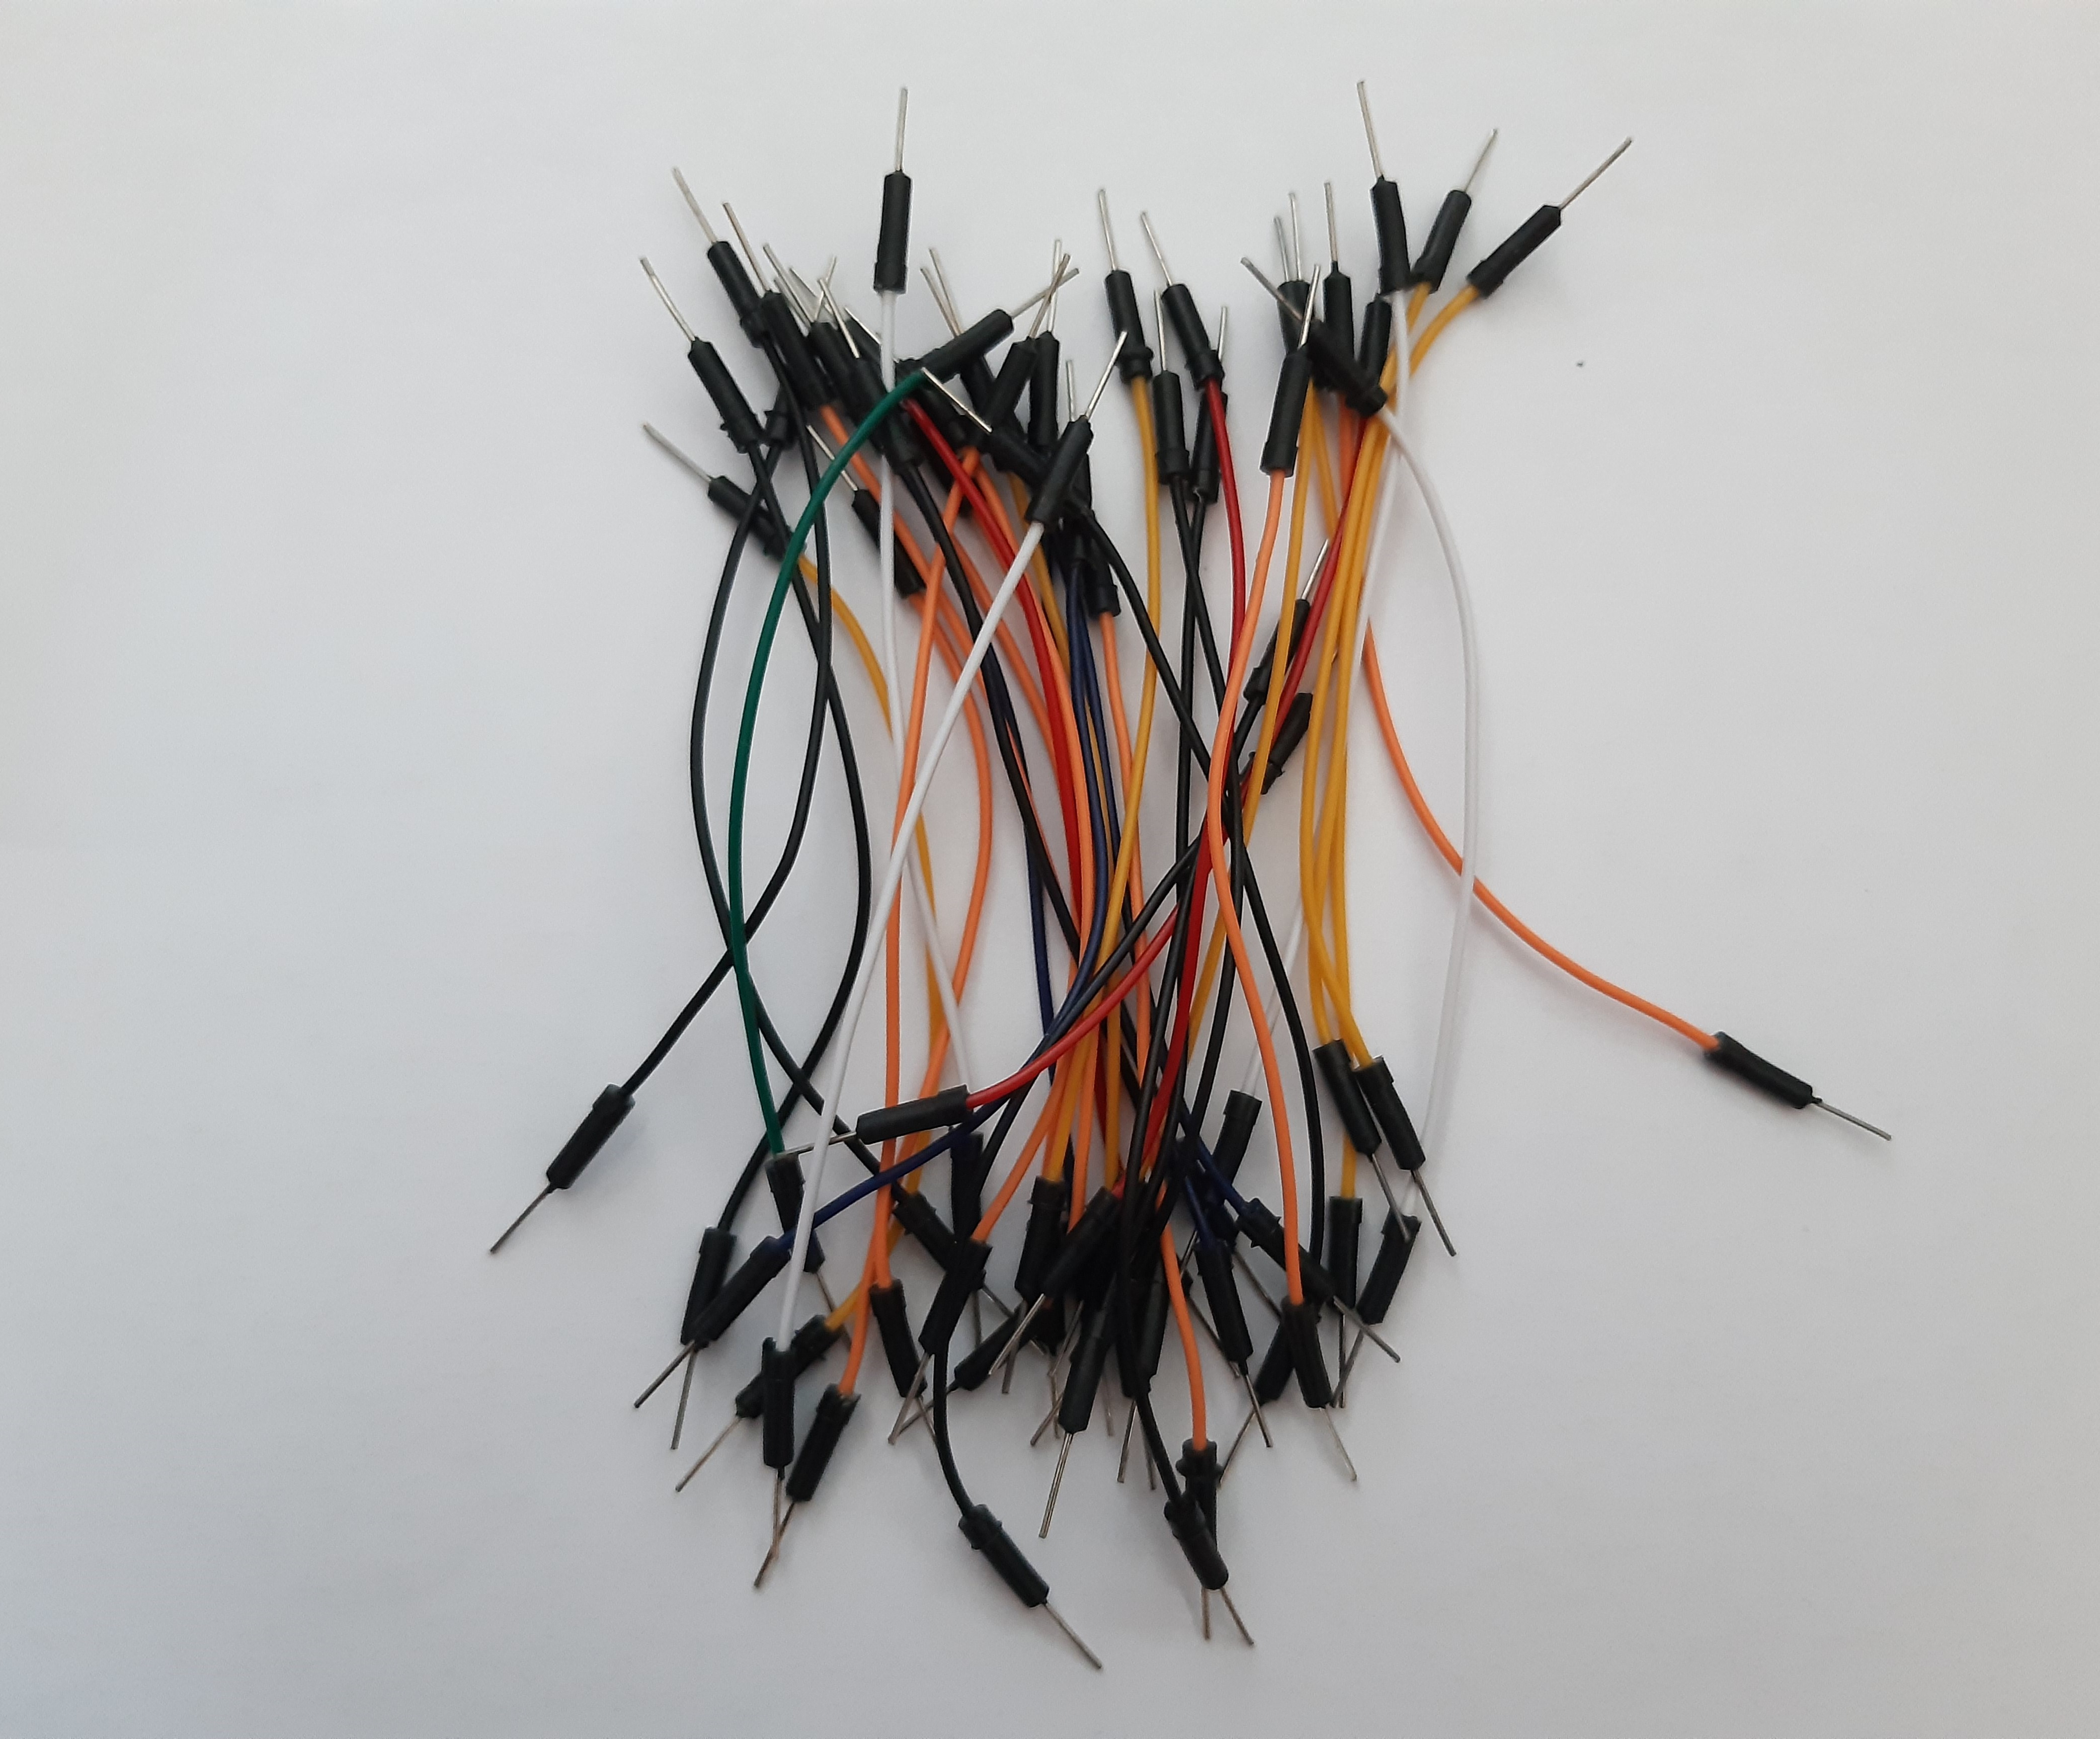
\includegraphics[width=0.4\textwidth]{img/imgCableado.JPG}
    \caption{Cables de conexiones para arduino.}
    \label{fig:cableado}
\end{figure}

\item \textbf{Resistencias}: componentes electrónicos que limitan el flujo de energía eléctrica del circuito. El valor de cada resistencia viene dado por un código de colores. En la \textit{Figura \ref{fig:resistencias}} se puede ver una imagen del componente.
% Imagen de las resistencias.
\begin{figure}[h!]
    \centering
    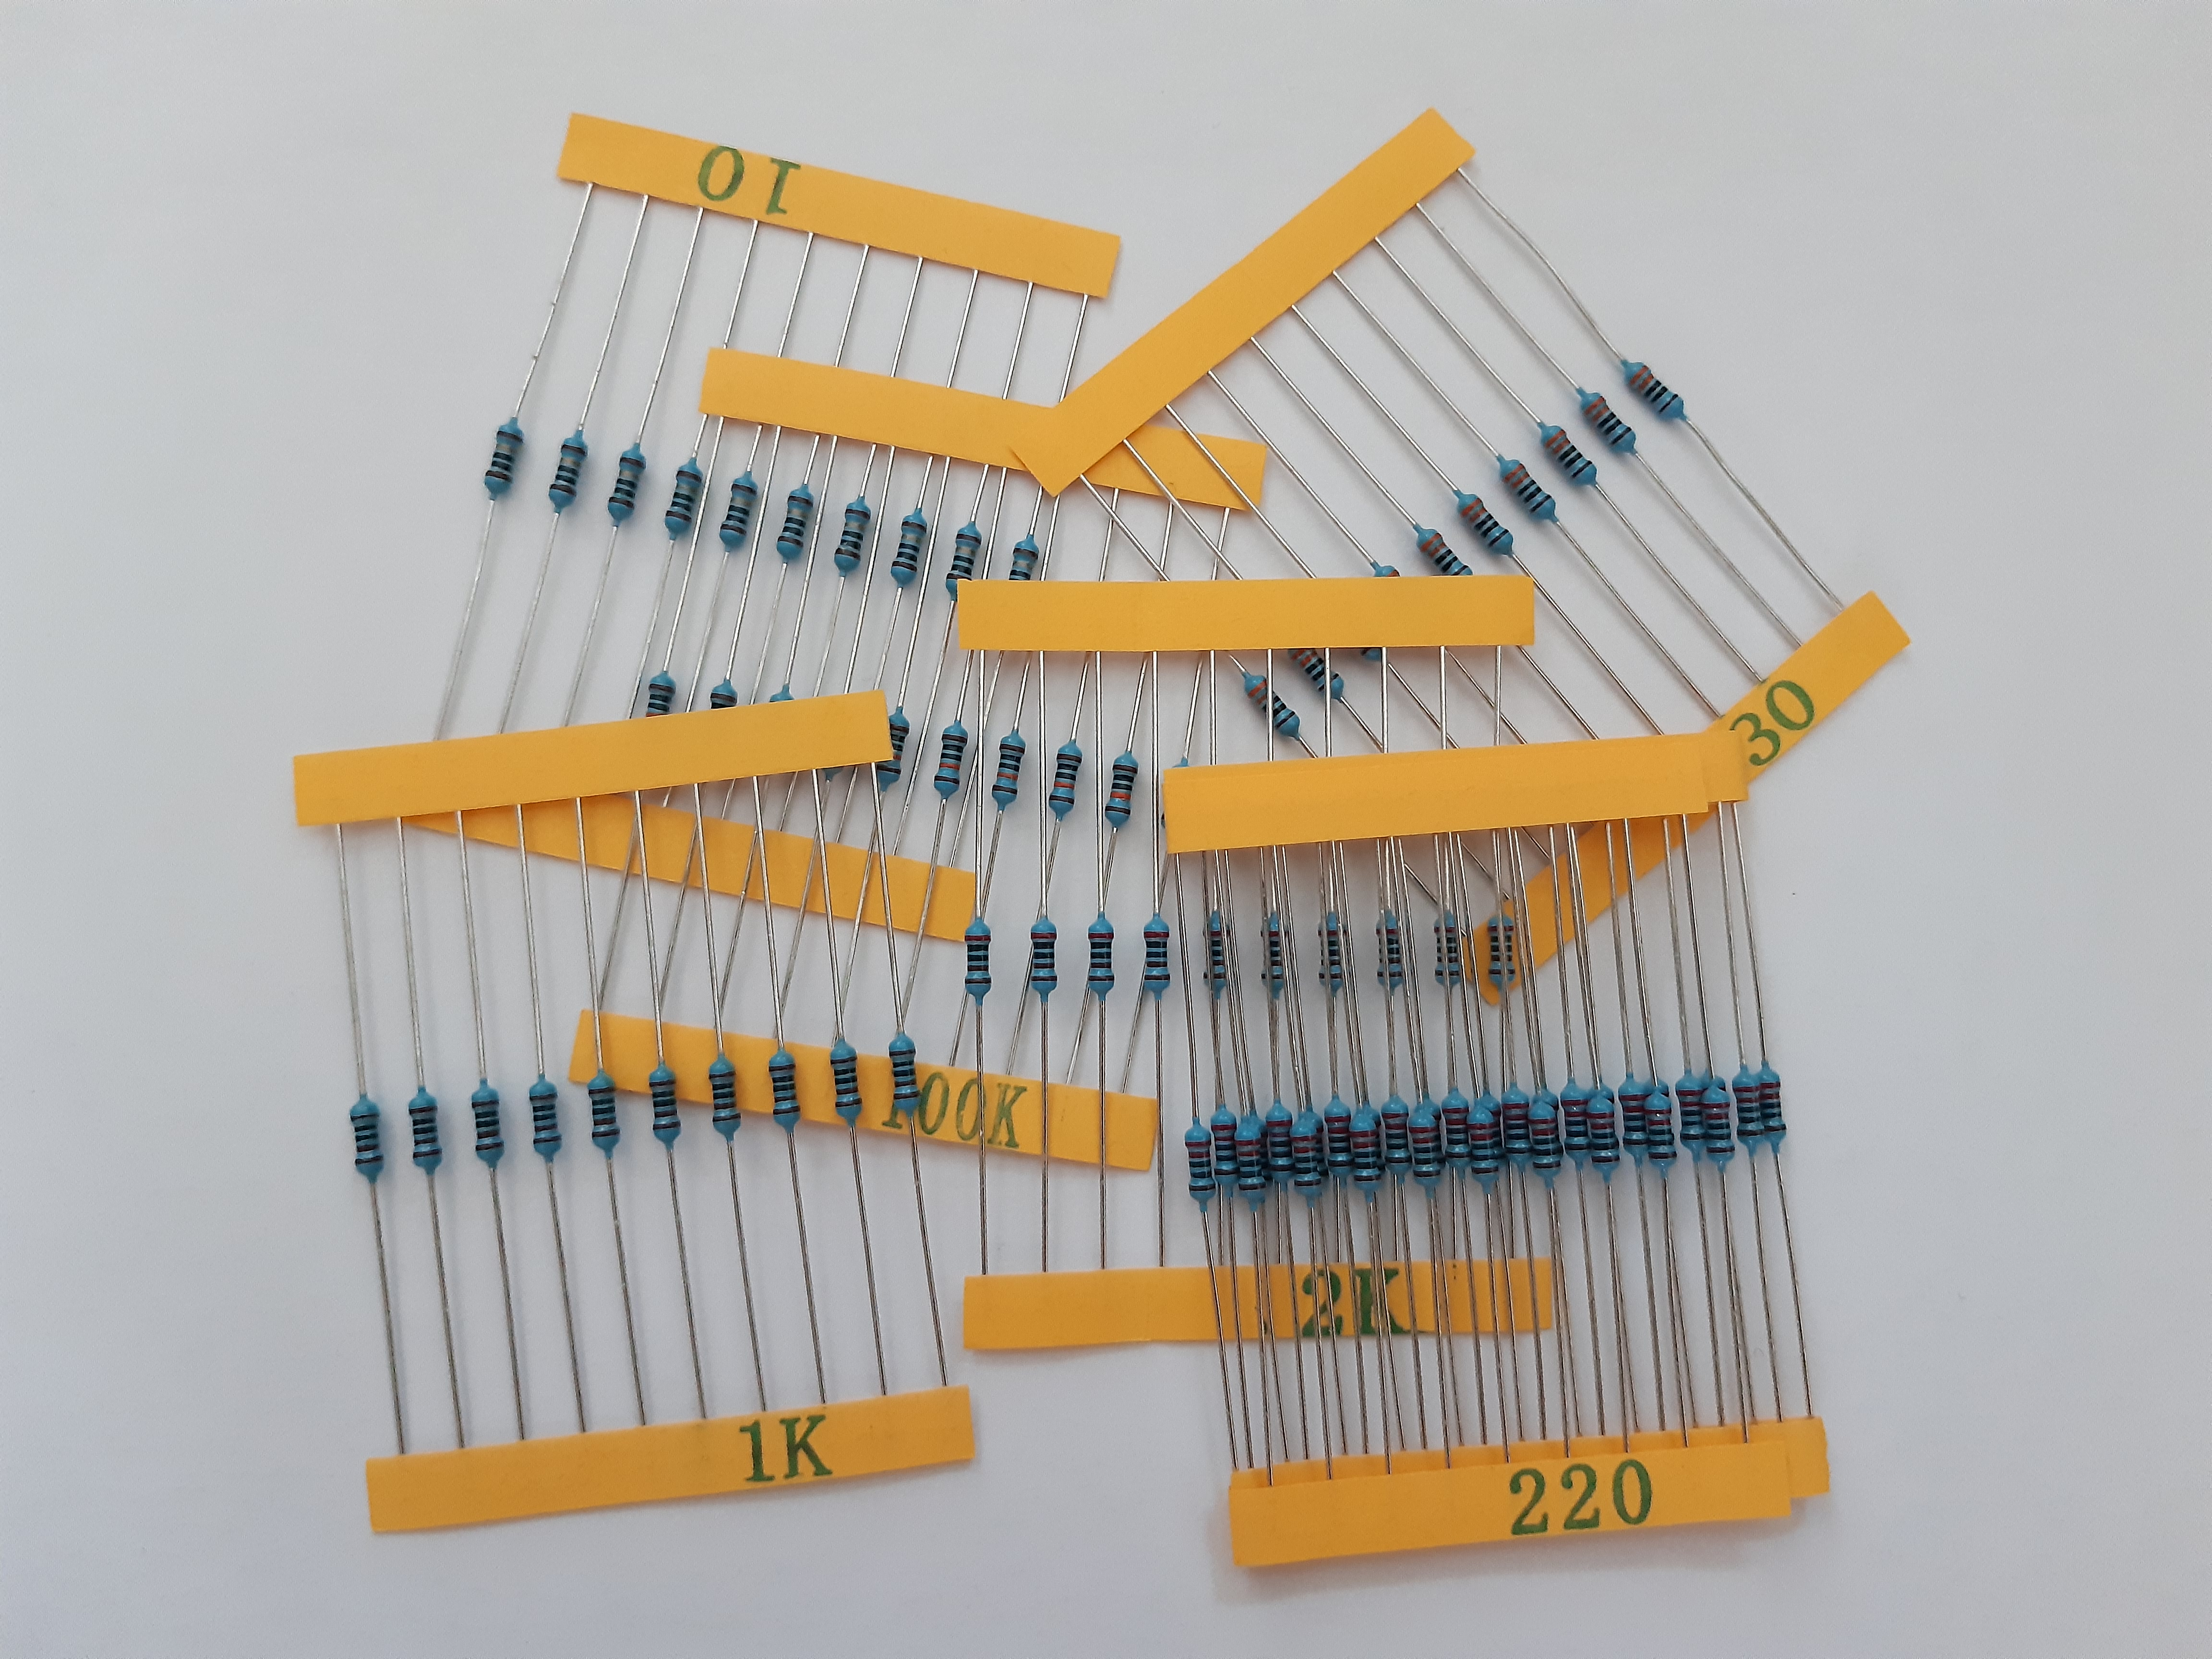
\includegraphics[width=0.5\textwidth]{img/imgResistencias.JPG}
    \caption{Distintas resistencias. Fuente Propia.}
    \label{fig:resistencias} 
\end{figure}

\item \textbf{Leds}: diodo que se ilumina cuando pasa una corriente eléctrica por él. Existen leds de diferentes colores. En la \textit{Figura \ref{fig:leds}} se puede ver una imagen del componente.
% imagen de los leds
\begin{figure}[h!]
    \centering
    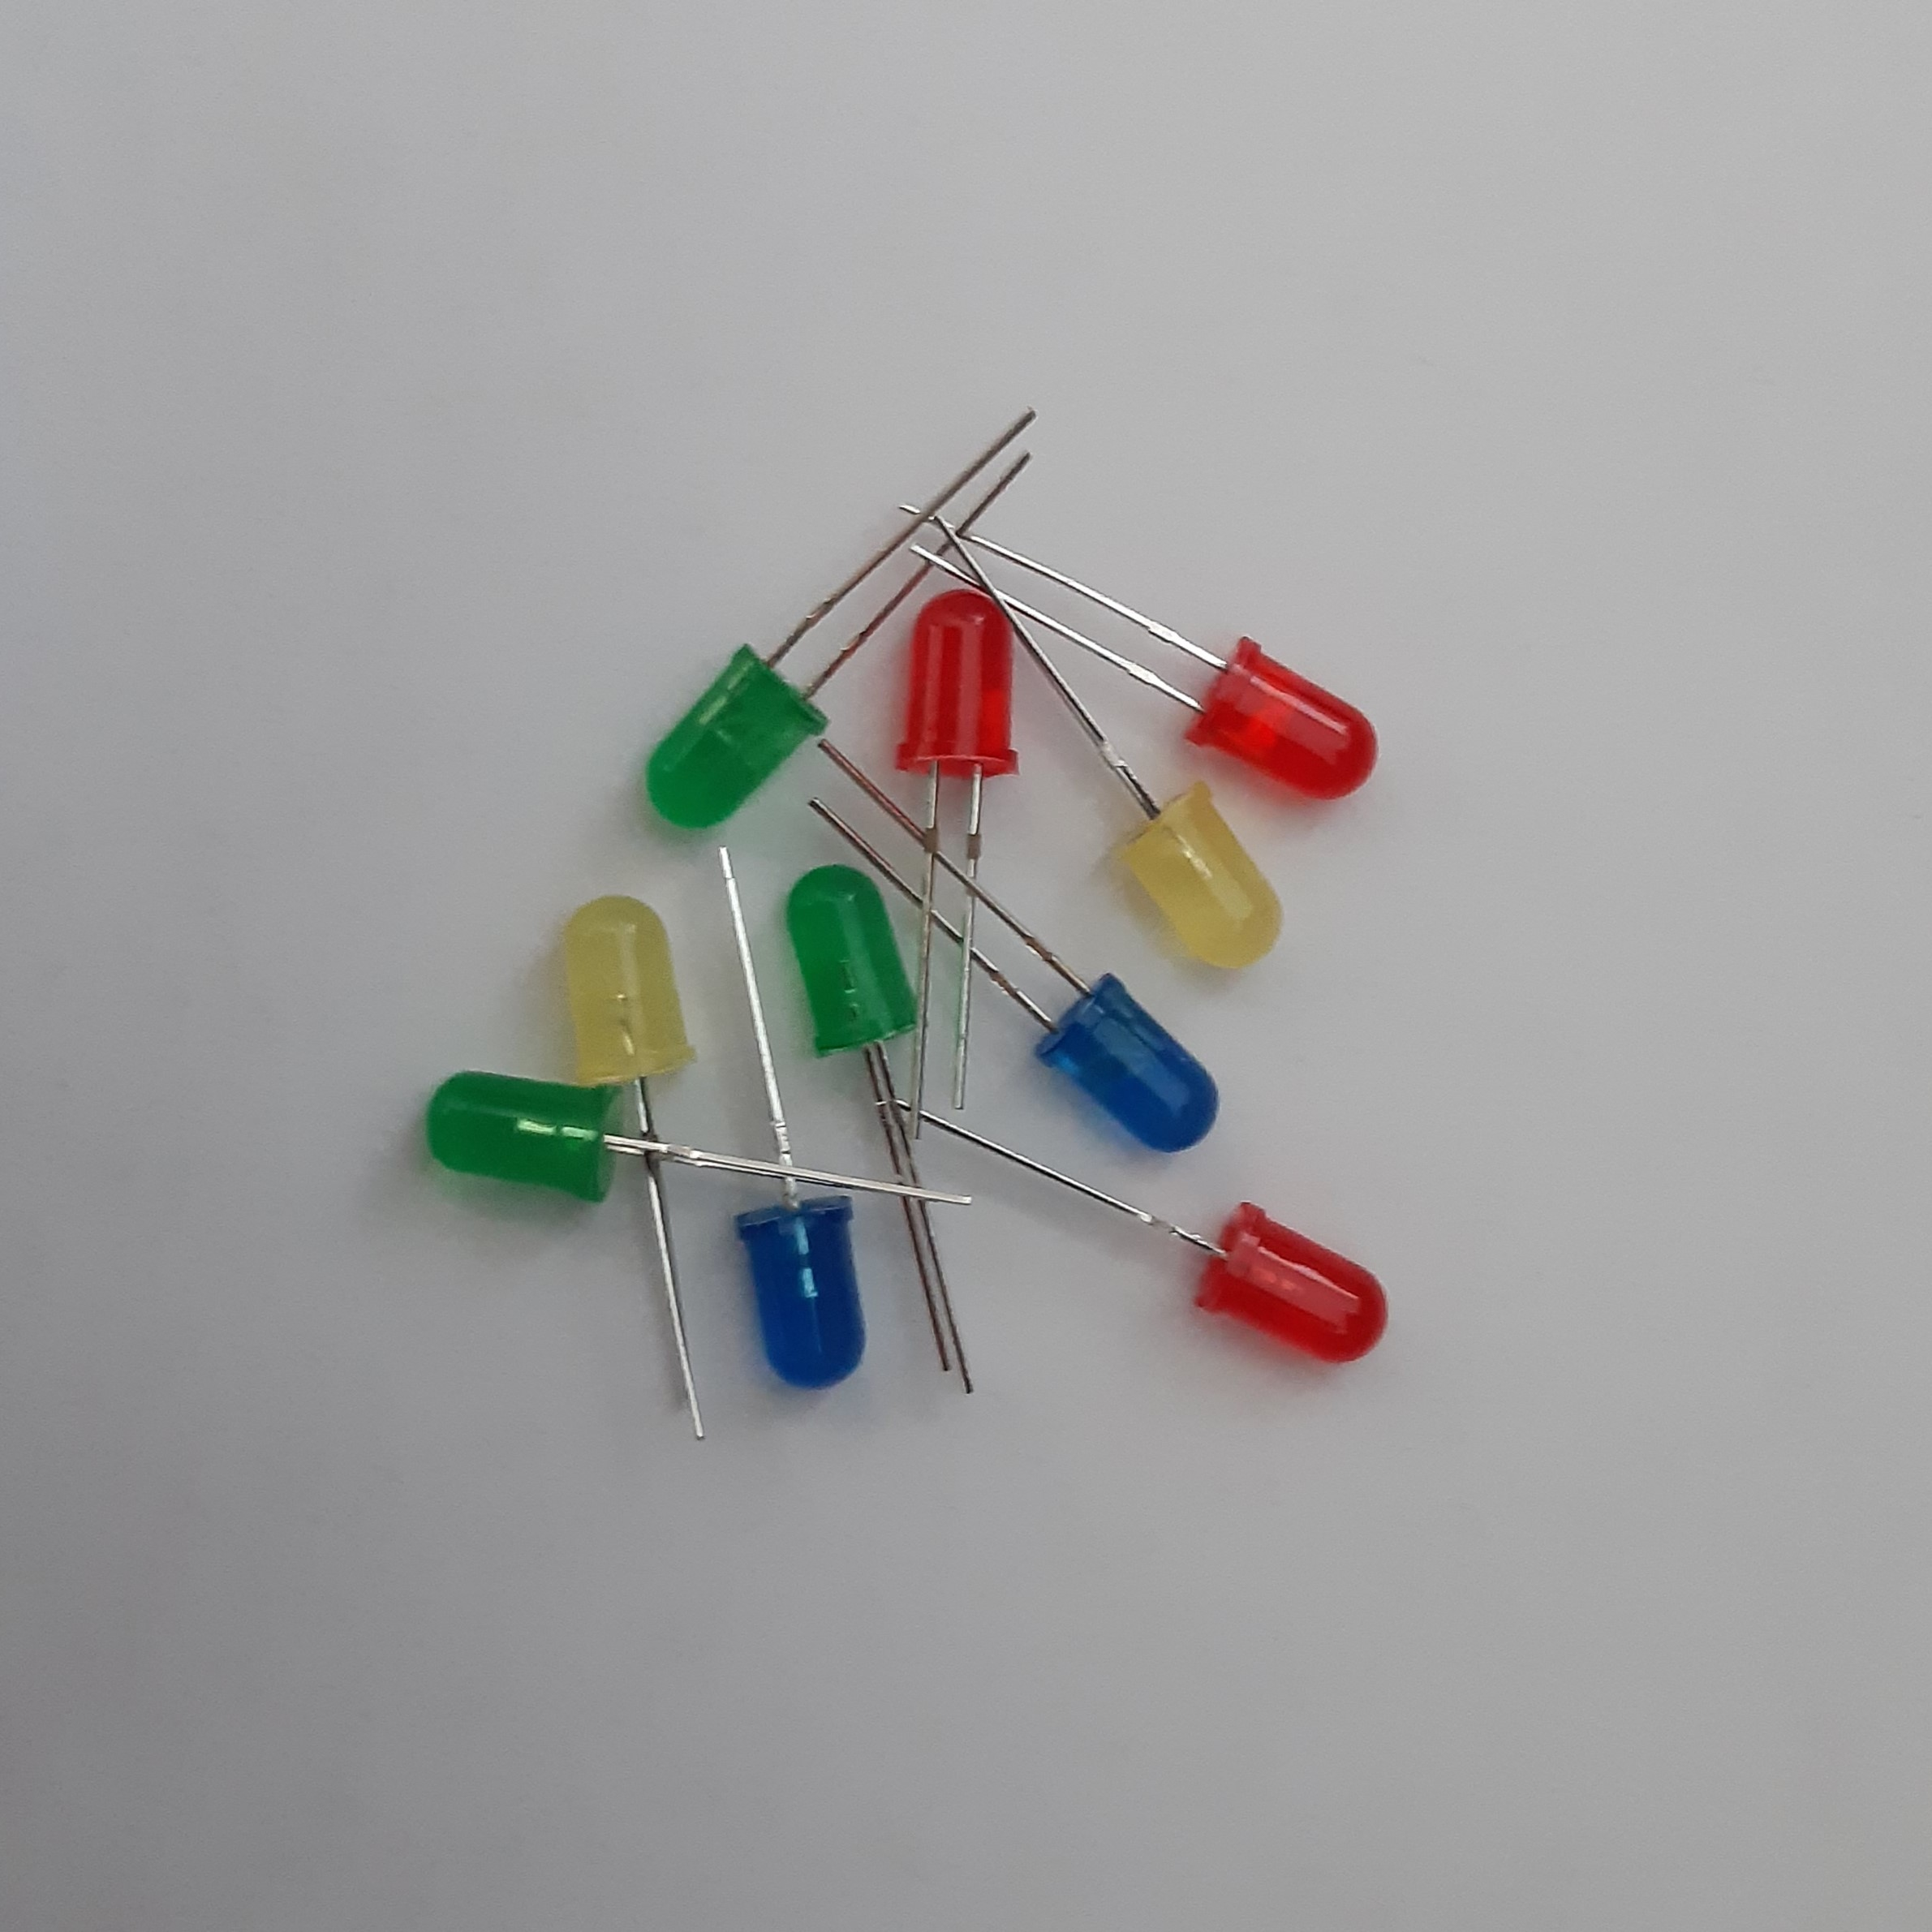
\includegraphics[width=0.4\textwidth]{img/imgLeds.JPG}
    \caption{Leds de diferentes colores. Fuente Propia.}
    \label{fig:leds} 
\end{figure}

\item \textbf{Pulsador}: componente que según su estado permite cortar o admitir el paso de corriente. En función de su estado se realizará una acción específica u otra. En la \textit{Figura \ref{fig:pulsador}} se puede ver una imagen del componente.
% Imagen de pulsadores de arduino
\begin{figure}[h!]
    \centering
    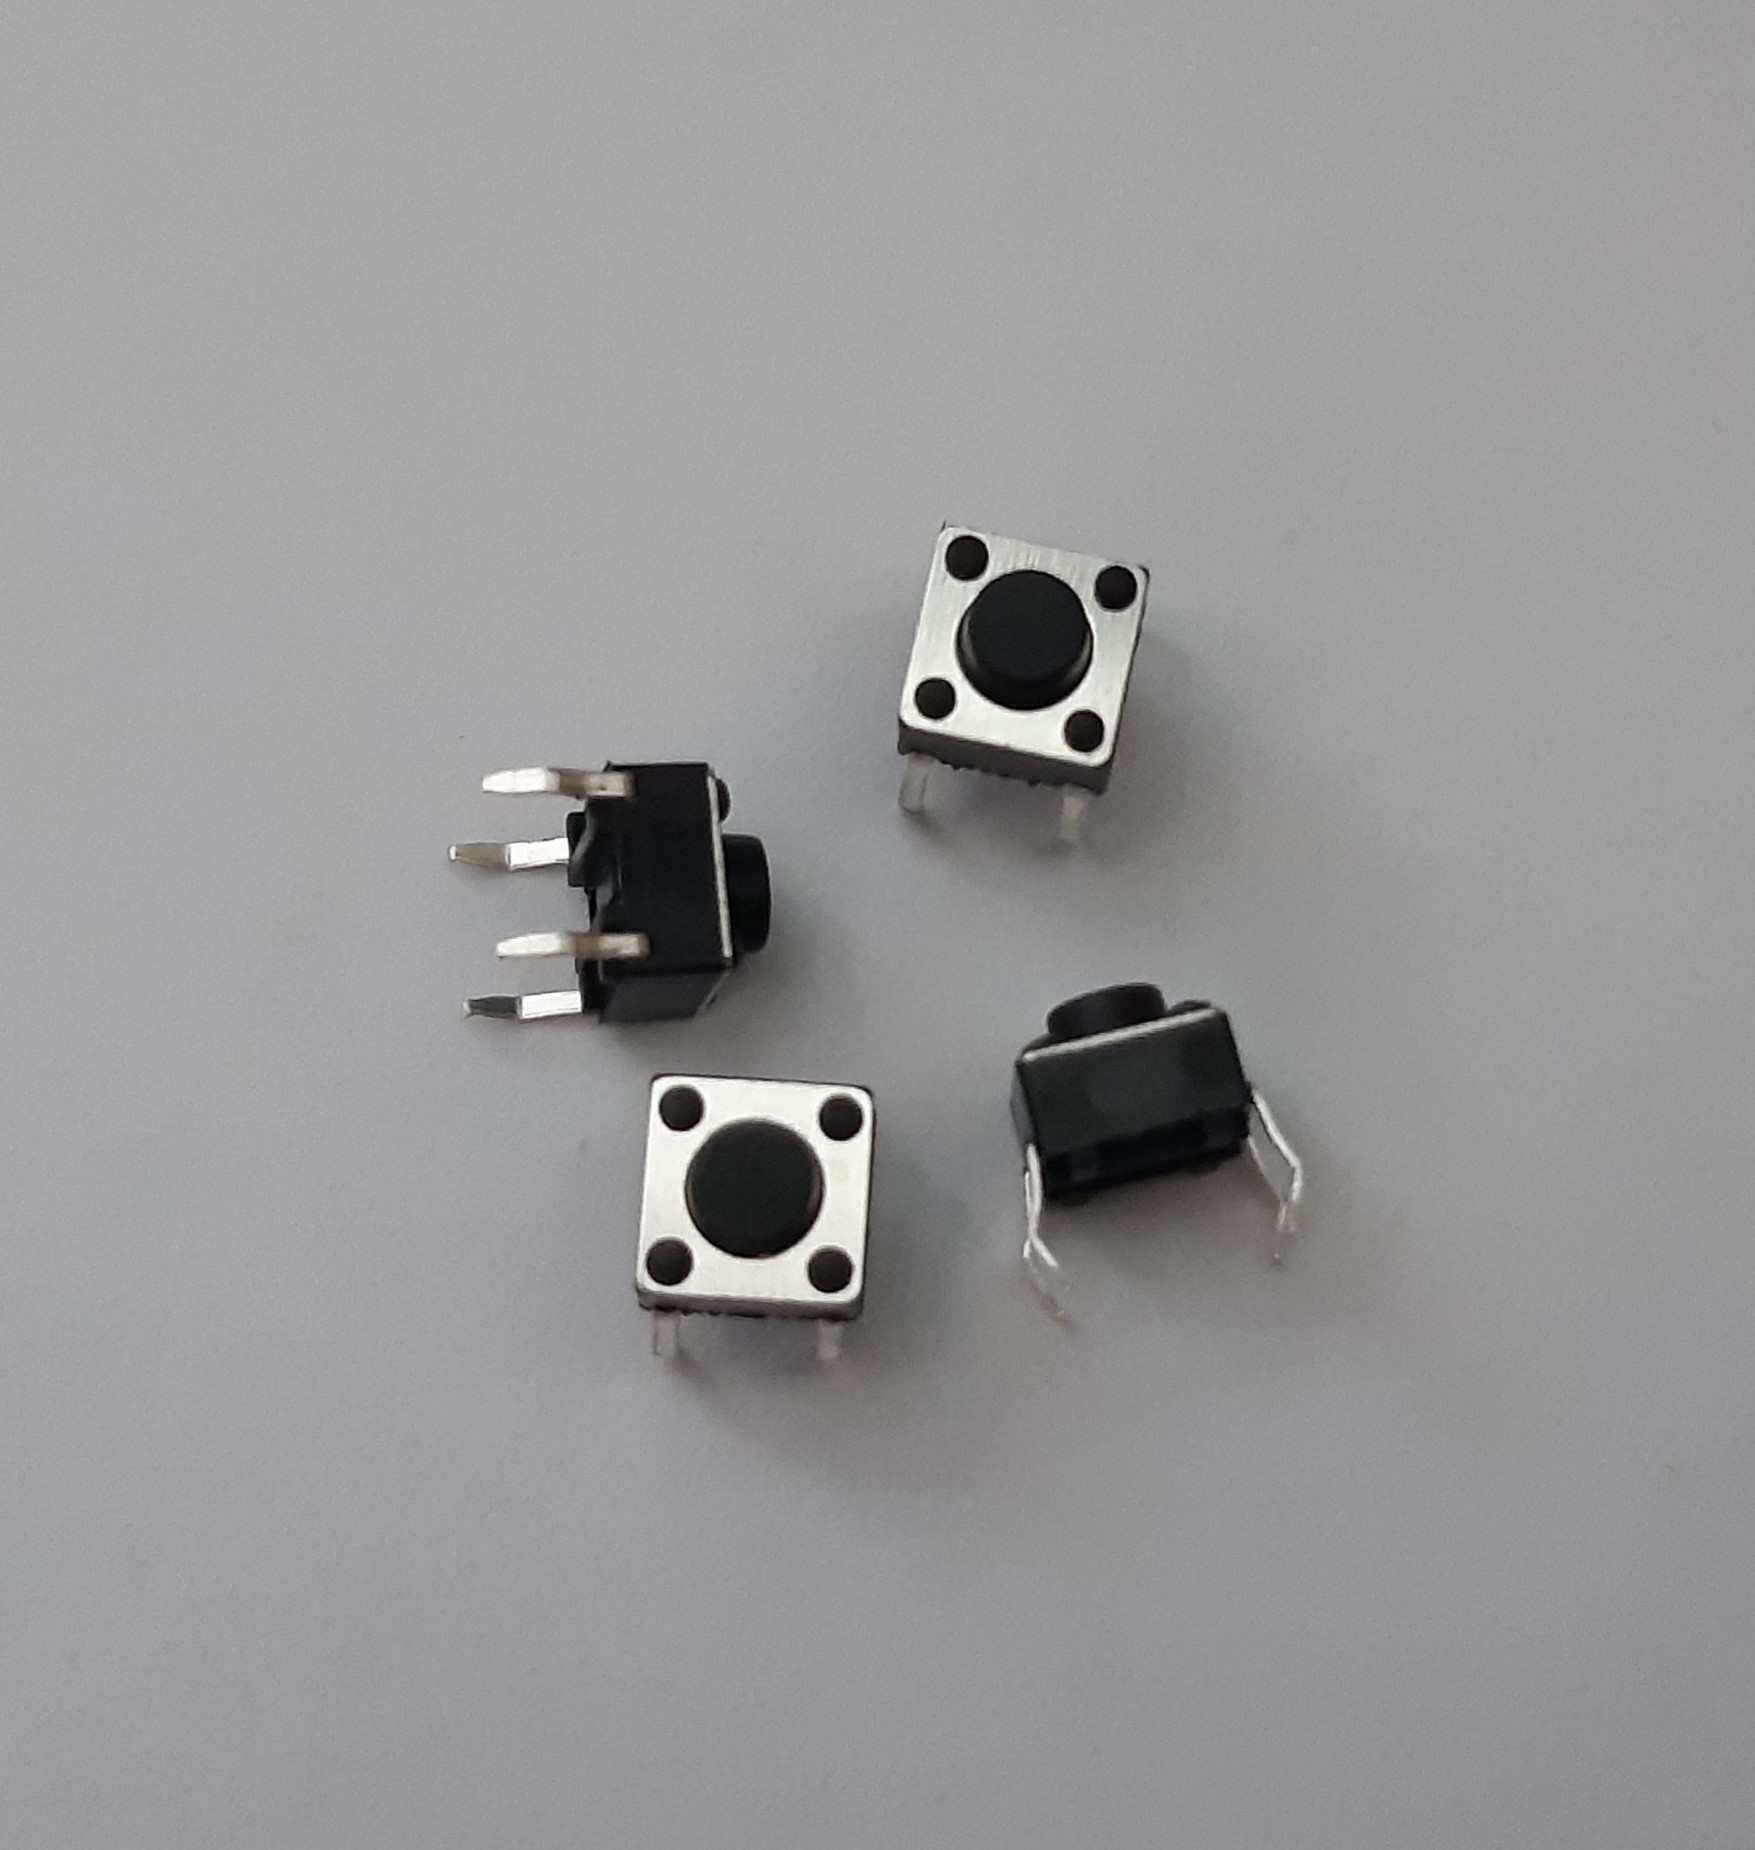
\includegraphics[width=0.4\textwidth]{img/imgPulsador.JPG}
    \caption{Pulsadores. Fuente Propia.}
    \label{fig:pulsador} 
\end{figure}

\item \textbf{Cable USB}: conector que permite introducir las instrucciones programadas en un ordenador a la placa de Arduino. En la \textit{Figura \ref{fig:cableUSB}} se puede ver una imagen del componente.
% Imagen del cable USB que conecta el arduino
\begin{figure}[h!]
    \centering
    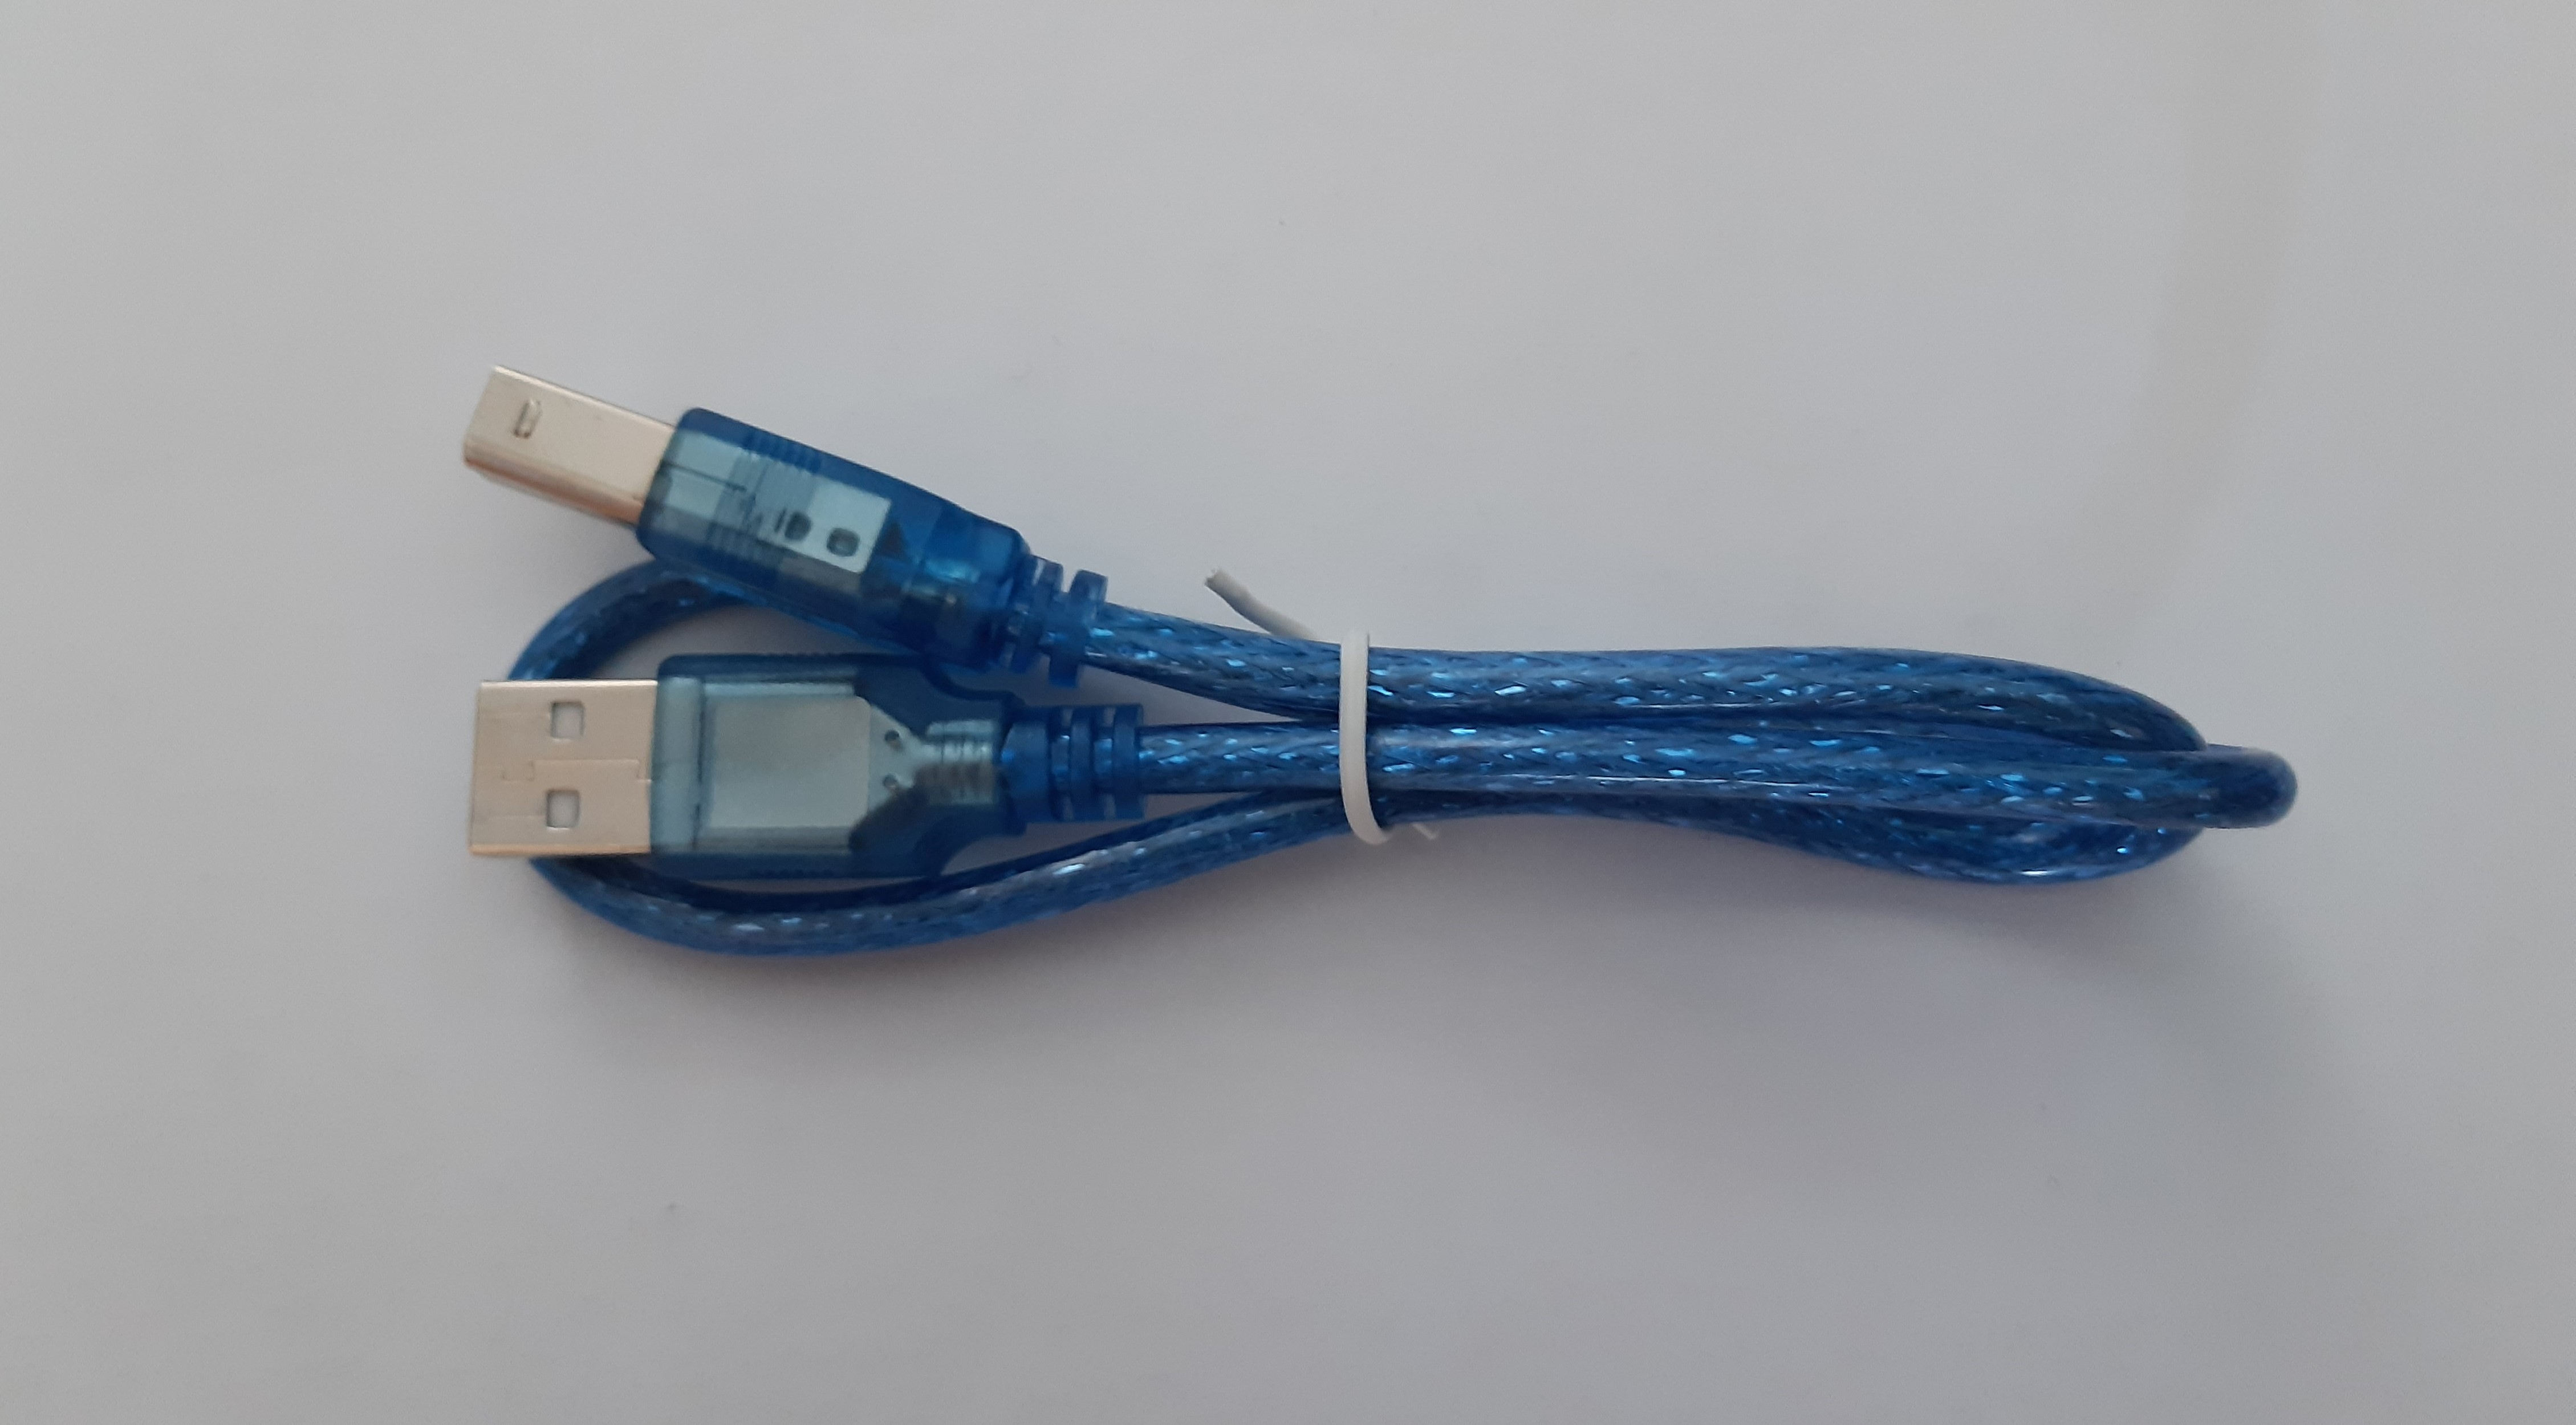
\includegraphics[width=0.5\textwidth]{img/imgCableUSB.JPG}
    \caption{Cable USB. Fuente Propia.}
    \label{fig:cableUSB} 
\end{figure}

\item \textbf{Motor de vibración}: componente electrónico que al alimentarlo causa un efecto vibratorio. En este proyecto su finalidad será la de alertar al usuario mediante un biofeedback de señal vibratoria. En la \textit{Figura \ref{fig:motorVibr}} se puede ver una imagen del componente.
% Imagen de un motor de vibración
\begin{figure}[h!]
    \centering
    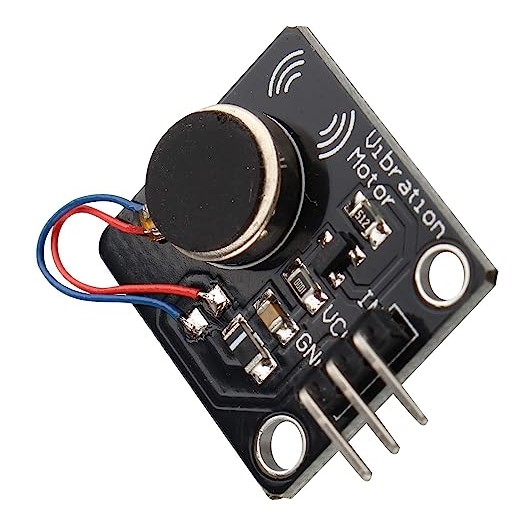
\includegraphics[width=0.4\textwidth]{img/MotorVibr.jpg}
    \caption{Motor de vibración.\cite{imgMotorVibr}}
    \label{fig:motorVibr} 
\end{figure}

\newpage
\item \textbf{Zumbador pasivo}: un transductor electroacústico que transforma una señal acústica en un efecto sonoro. En este proyecto su finalidad será la de alertar al usuario mediante un biofeedback de señal sonora. En la \textit{Figura \ref{fig:zumbador}} se puede ver una imagen del componente.
% Imagen de un zumbador pasivo.
\begin{figure}[h!]
    \centering
    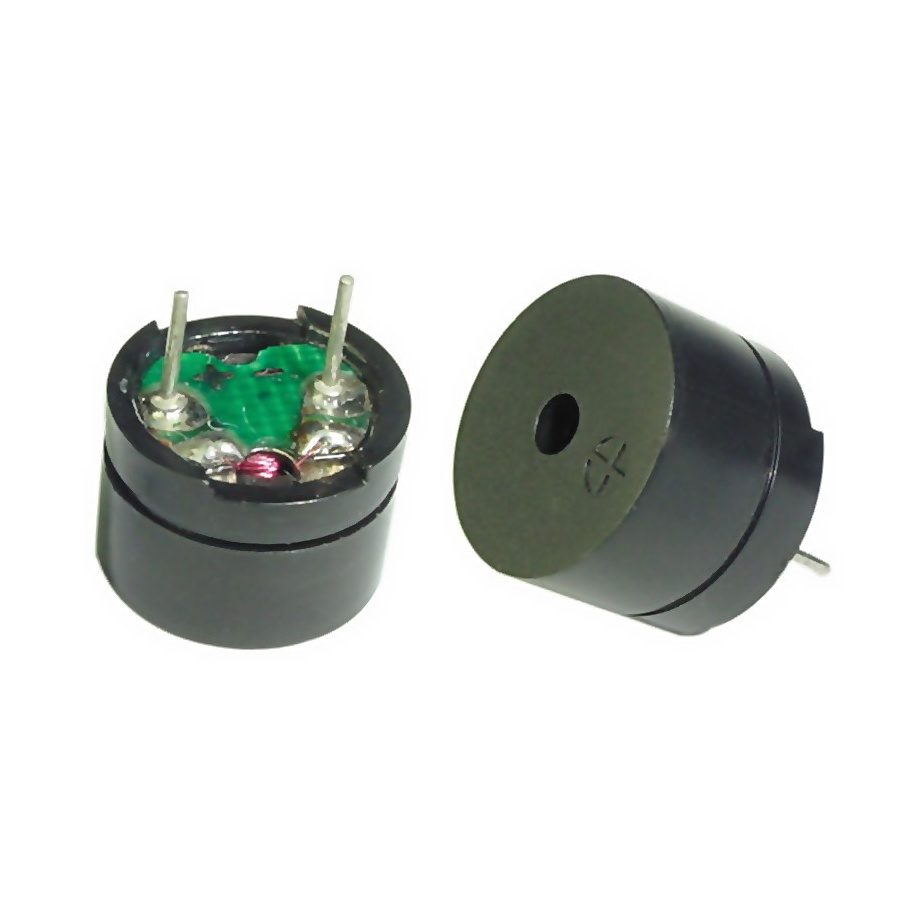
\includegraphics[width=0.4\textwidth]{img/imgZumbador.jpg}
    \caption{Zumbador pasivo.\cite{imgZumbador}}
    \label{fig:zumbador} 
\end{figure}

\end{itemize}

\newpage
\subsubsection{Posibles sensores.}

Se han estudiado distintos sensores que podrían ser empleados en los prototipos.

\begin{itemize}
    \item \textbf{Módulo SCA60C}\cite{SCA60C}: módulo que consta de un sensor de ángulo SCA60C y un acelerómetro N100060. Gracias a este sensor se pueden medir ángulos de 0 a 180º, con resolución de un grado, con un voltaje de entrada de 5 voltios y una tensión de salida en función del ángulo de 0,45 - 4,5 voltios. La corriente que necesita el módulo ronda los 2 mA. Este módulo admite distintos rangos de medición y se utiliza para multitud de aplicaciones en las que se necesite conocer constantemente el ángulo de giro. En la \textit{Figura \ref{fig:SCA60C}} se puede ver una imagen del sensor.
% Imagen Módulo SCA60C
\begin{figure}[h!]
    \centering
    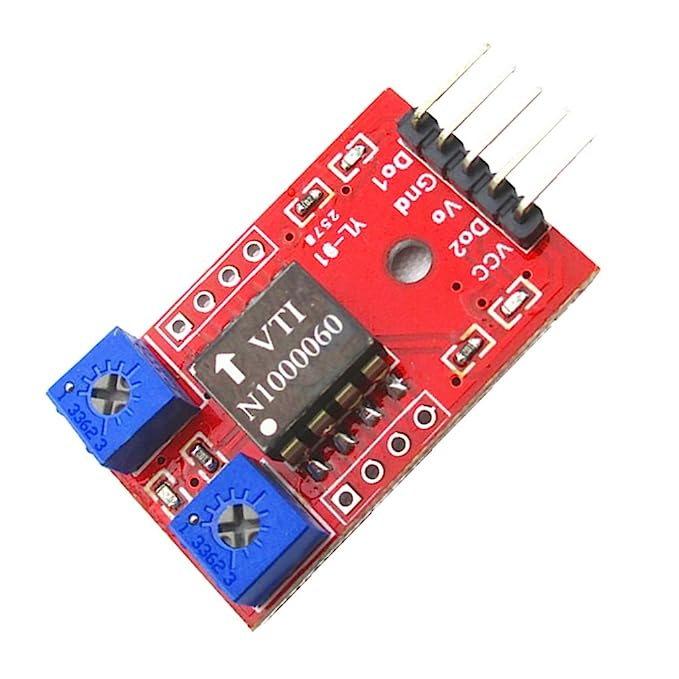
\includegraphics[width=0.3\textwidth]{img/imgSCA60C.jpg}
    \caption{Módulo SCA60C\cite{imgSCA60C}.}
    \label{fig:SCA60C} 
\end{figure}
    
    \item \textbf{Galgas extensiométricas y módulo HX711}\cite{GyHX711_1,GyHX711_2}: se trata de un conjunto cuyo objetivo es medir el peso, basado en un transductor de galgas extensiométricas y un módulo HX711 que actúa como amplificador de la señal y transfiere los datos al microcontrolador. La galga extensiométrica o celda de carga es un transductor que convierte la tensión generada por los cambios en la longitud de un objeto a una señal eléctrica, en función del peso que se quiere medir existen distintas celdas de carga. Mientras que el módulo HX711 consta de un amplificador y un convertidor analógico-digital, que permite la amplificación de la señal producida por la galga extensiométrica. Este módulo utiliza un puente de Weahstone para convertir la fuerza aplicada en una señal analógica. Necesita una tensión de entrada de 5 voltios y el resultado se puede obtener en g, kg o Newtons. La utilización de este módulo requiere de la librería de Arduino hx711. El precio ronda los 10-15€. En la \textit{Figura \ref{fig:HX711}} se puede ver una imagen del conjunto.
% Imagen de galgas extensiometricas y el módulo HX711
\begin{figure}[h!]
    \centering
    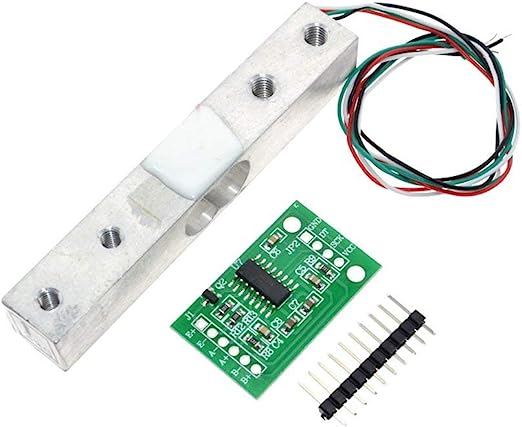
\includegraphics[width=0.3\textwidth]{img/GyHX711.jpg}
    \caption{Galgas extensiométricas y módulo HX711\cite{imgGyHX711}.}
    \label{fig:HX711} 
\end{figure}

    \item \textbf{Acelerómetro ADXL345}\cite{ADXL345}: acelerómetro micromecanizado (MEMS) capacitivo de 3 grados de Libertad (3DOF\footnote{\textbf{DOF: Degrees of Freedom, los grados de libertad, hace referencia a la cantidad de ejes en los que un sensor puede realizar su medición}}) acoplado a un bloque de memoria FIFO que almacena hasta 32 conjuntos de coordenadas. Además, es compatible con un procesador como Arduino mediante conexión por bus SPI o bus I2C. Este dispositivo permite conocer la orientación del sensor por la acción de la fuerza de gravedad basándose en la detección de la aceleración en los ejes X, Y y Z. Se trata de un dispositivo de ultra bajo consumo, únicamente consume en funcionamiento unos 45 $\mu$A de corriente mientras que en Stand-By solamente consume unos 0,1 $\mu$A. Este acelerómetro necesita una tensión de alimentación de unos 2 a 3,6 voltios. El rango de medición del dispositivo es ajustable, con resolución de hasta 13 bits y sensibilidad de 40 mg/LBS. En la \textit{Figura \ref{fig:ADXL345}} se puede ver una imagen del sensor.
% Imagen del acelerómetro ADXL345
\begin{figure}[h!]
    \centering
    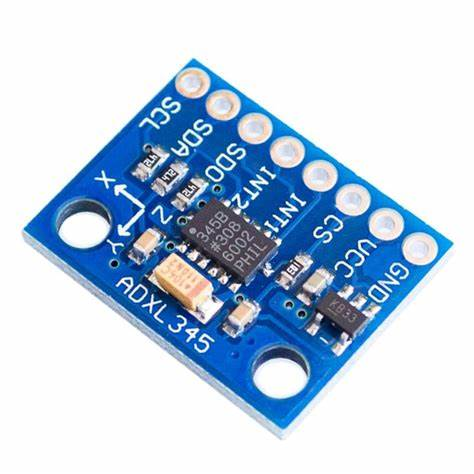
\includegraphics[width=0.2\textwidth]{img/ADXL345.jpeg}
    \caption{Acelerómetro ADXL345\cite{imgADXL345}.}
    \label{fig:ADXL345} 
\end{figure}

    \item \textbf{Módulo SW520D}\cite{SW520D_1}: Sensor de inclinación formado por sensores Tilt de doble esfera. Este sensor funciona como un intrerruptor y tiene una salida digital. Al inclinar el sensor las 2 esferas actúan de puente y cierran el circuito, se puede ver su diagrama en la \textit{Figura \ref{fig:imgSW520D}}. El código de programación de este dispositivo es similar al de un interruptor. Se trata de un sensor muy sensible a movimientos bruscos y vibraciones. Sin embargo, es un sensor muy barato. En la \textit{Figura \ref{fig:SW520D}} se pueden consultar las conexiones.
    % Referencia: 
    % https://www.luisllamas.es/medir-inclinacion-con-arduino-y-sensor-tilt-sw-520d/
% Imagen del sensor SW520D
\begin{figure}[h!]
    \centering
    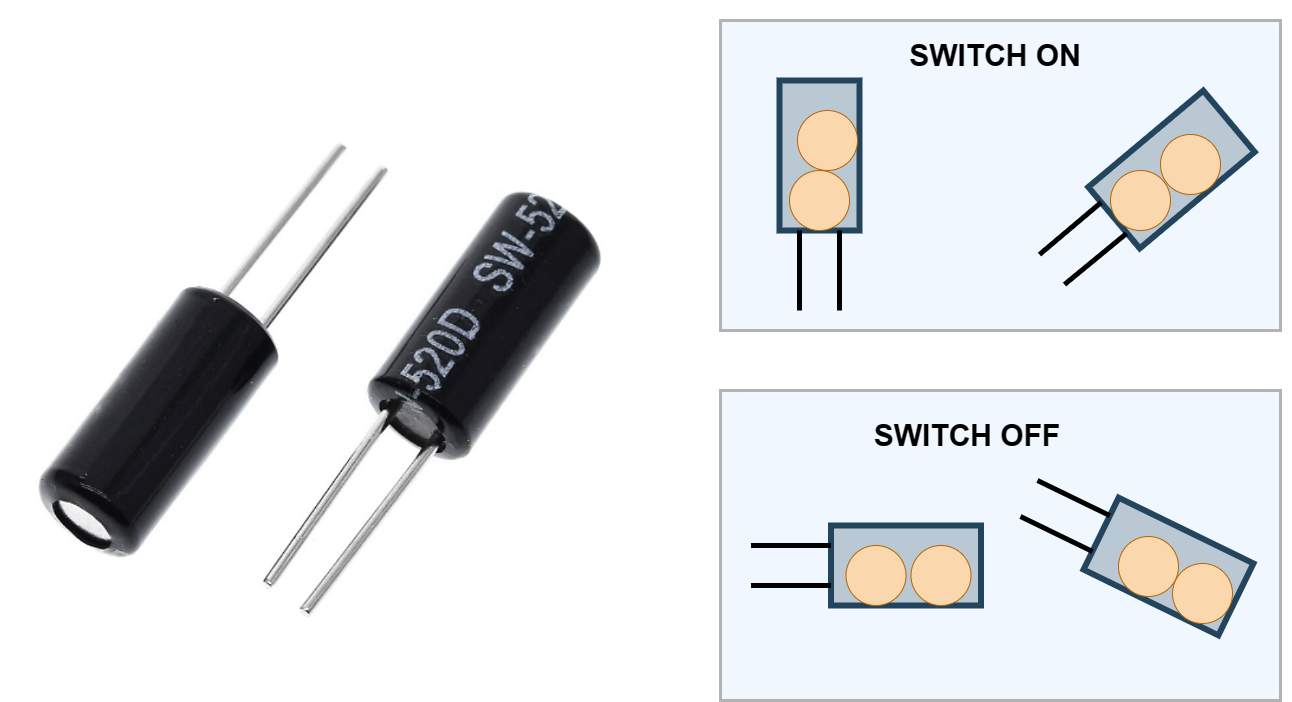
\includegraphics[width=0.4\textwidth]{img/imgSW520D_diag.png}
    \caption{Sensor SW520D\cite{imgSW520D} y diagrama de su funcionamiento.}
    \label{fig:imgSW520D} 
\end{figure}

% Diagrama del sensor SW520D
\begin{figure}[h!]
    \centering
    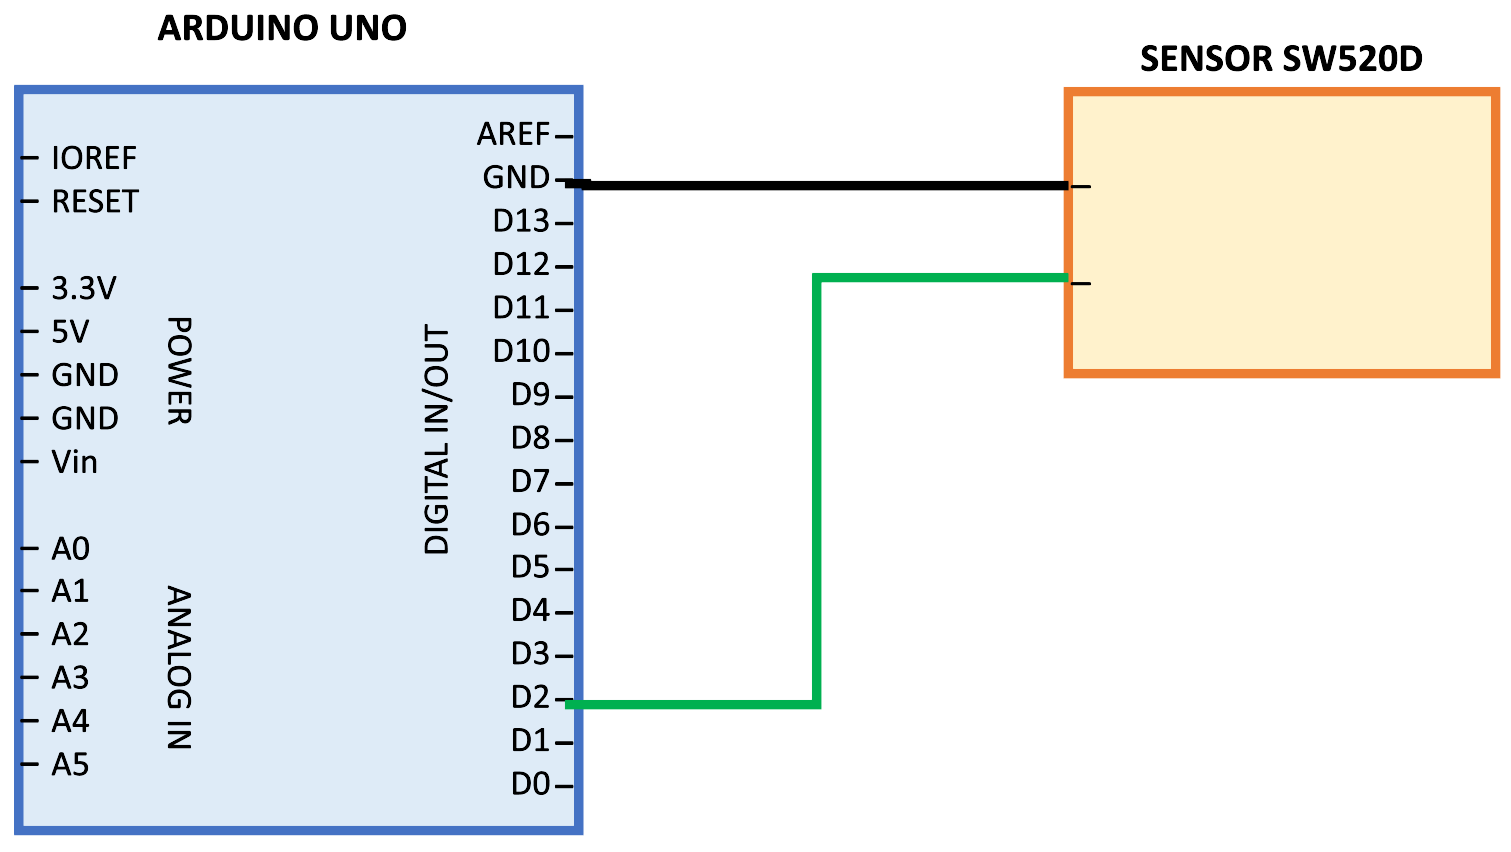
\includegraphics[width=0.5\textwidth]{img/SW520D.png}
    \caption{Diagrama de las conexiones del sensor SW520D. Fuente Propia.}
    \label{fig:SW520D} 
\end{figure}

    \item \textbf{IMU MPU-6050}\cite{MPU6050_1,MPU6050_2}: es un módulo de unidad de medición inercial de 6 grados de libertad (6 DOF) fabricado por Invensense\cite{invensense}, que permite conocer la posición del sensor en todo momento. Este módulo consta de un acelerómetro de 3 ejes, un giroscopio de 3 ejes, conversores analógico a digital (ADC) de 16 bits, un sensor de temperatura, un reloj de alta precisión e interrupciones programables y un procesador interno (DMP Digital Motion Porcessor). Tanto el rango del acelerómetro como del giroscopio son ajustables. Este módulo se acopla mediante un bus SPI o un bus I2C, necesita una tensión de alimentación de unos 2,4 - 3,6 voltios, aunque hay algunos módulos que tienen incluido un regulador de voltaje que permite su conexión a un voltaje de 5V, y consume unos 3,5 mA al tener todos sus componentes activados. Es uno de los sensores más empleados y tiene un coste de unos 6-15€. Para ver una imagen del sensor y sus conexiones ver \textit{Figura \ref{fig:imgMPU6050}} y \textit{Figura \ref{fig:MPU6050}}.
% Imagen del módulo MPU6050
\begin{figure}[h!]
    \centering
    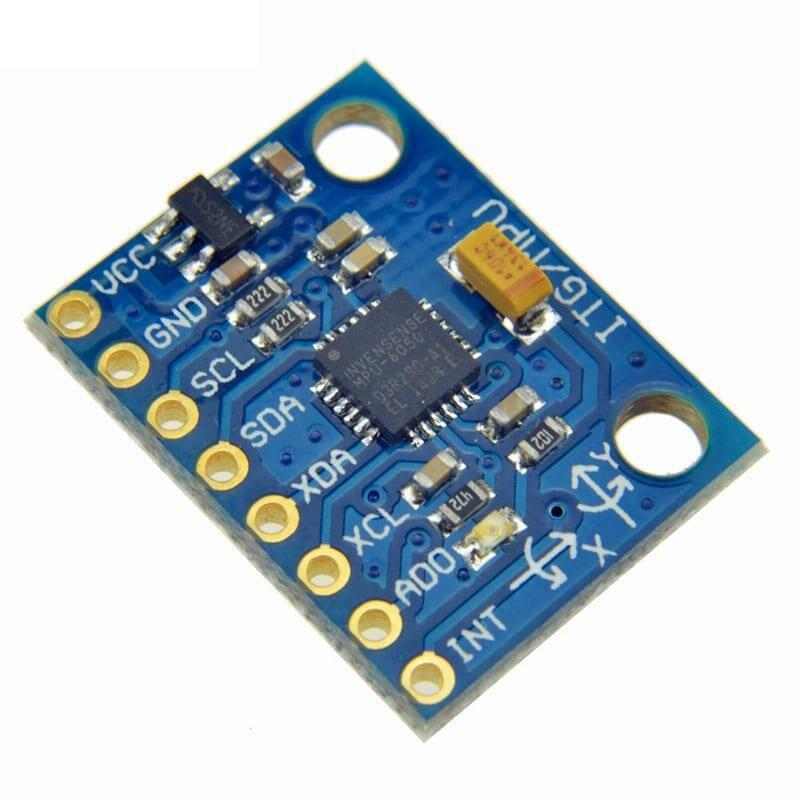
\includegraphics[width=0.2\textwidth]{img/imgMPU6050.jpg}
    \caption{Módulo MPU-6050\cite{imgMPU6050}.}
    \label{fig:imgMPU6050}
\end{figure}
% Diagrama del sensor MPU6050
\begin{figure}[h!]
    \centering
    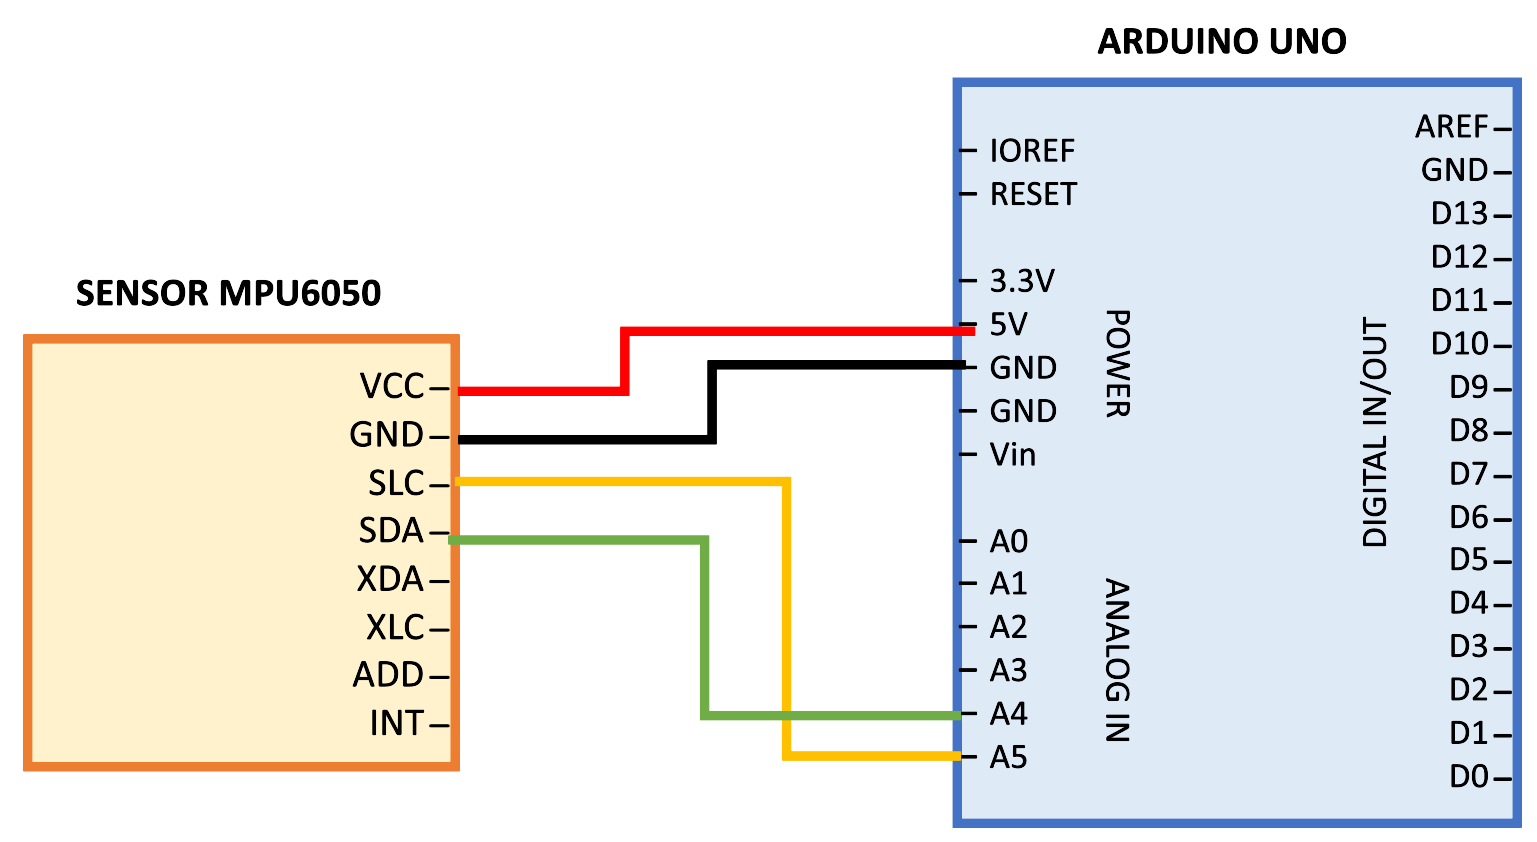
\includegraphics[width=0.5\textwidth]{img/MPU6050.png}
    \caption{Diagrama de las conexiones del módulo MPU6050 con regulador de voltaje. Fuente Propia.}
    \label{fig:MPU6050} 
\end{figure}

    \item \textbf{Módulo MPU-9250}\cite{MPU9250_1,MPU9250_2}: es un sensor de 9 grados de libertad (9DOF) que permite medir la inclinación y la aceleración en los 3 ejes. Este módulo incluye un acelerómetro, un giroscopio y un magnetómetro. Al incluir el magnetómetro se elimina la deriva que puede darse tras horas de uso en dispositivos que no tengan este componente. Además, este módulo se acopla mediante bus SPI o por bus I2C. Este sensor necesita una alimentación de entrada de unos 2.4 a 3.6 V, aunque hay algunos módulos que tienen incluido un regulador de voltaje que permite su conexión a un voltaje de 5V. Para programar este módulo es necesaria la librería de Arduino MPU9250\cite{libMPU9250}. Las figuras \textit{Figura \ref{fig:imgMPU9250}}, \textit{Figura \ref{fig:MPU9250}} y \textit{Figura \ref{fig:MPU9250R}} muestran una imagen del módulo y sus conexiones.
% Imagen del módulo MPU9250
\begin{figure}[h!]
    \centering
    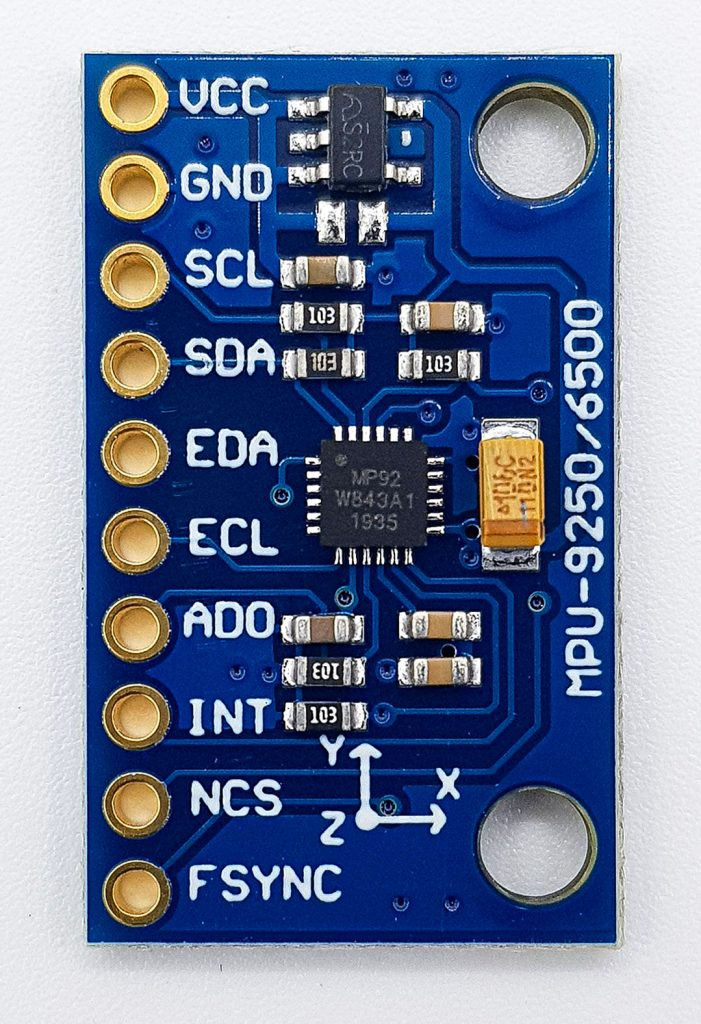
\includegraphics[width=0.15\textwidth]{img/imgMPU9250.jpg}
    \caption{Módulo MPU-9250\cite{imgMPU9250}.}
    \label{fig:imgMPU9250} 
\end{figure}

% Diagramas del sensor MPU9250
\begin{figure}[h!]
    \centering
    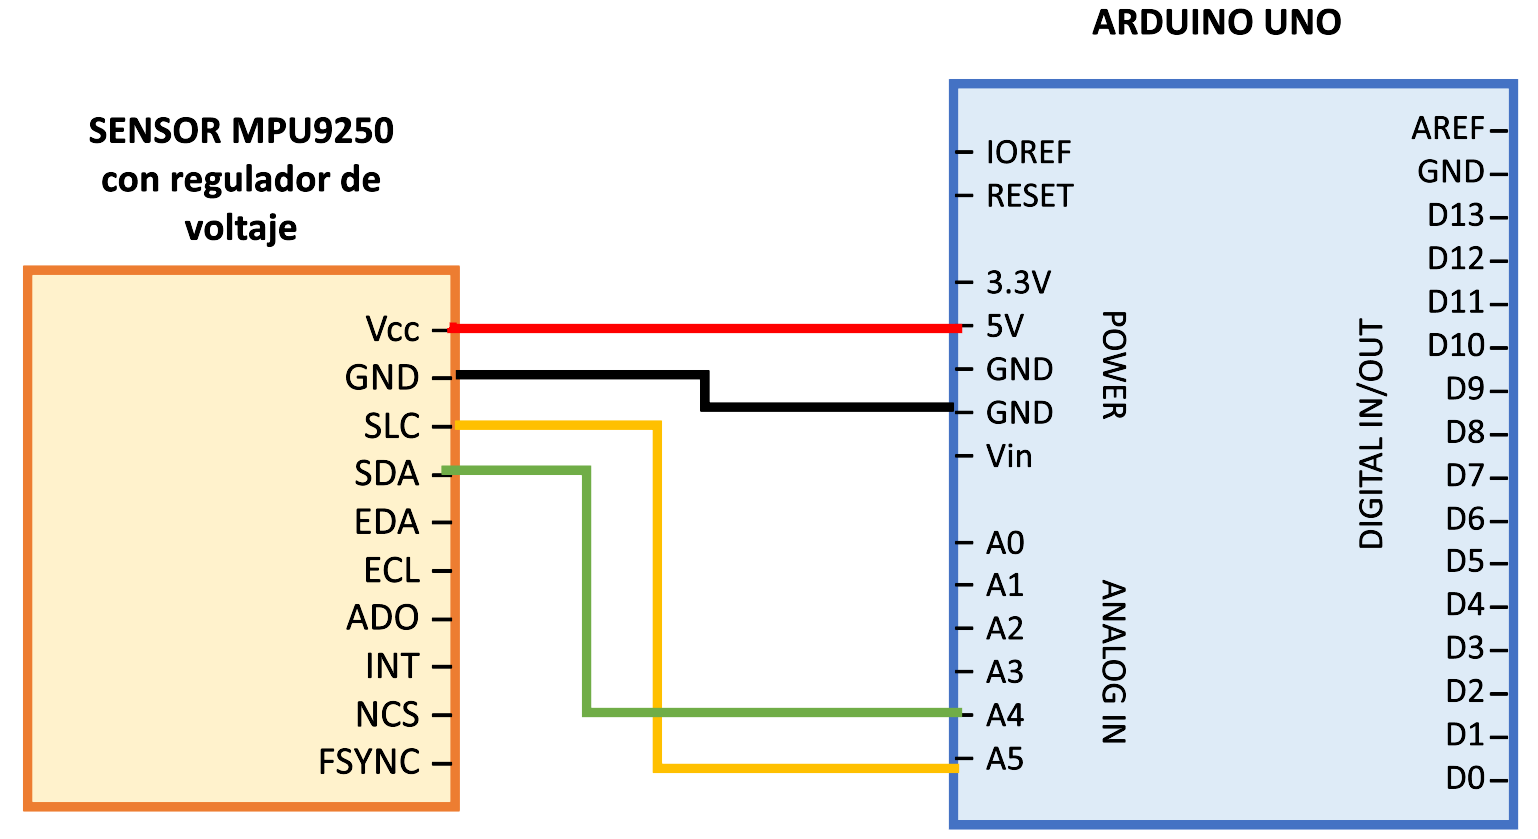
\includegraphics[width=0.5\textwidth]{img/MPU9250Regulador.png}
    \caption{Diagrama del módulo MPU9250 con regulador de voltaje. Fuente Propia.}
    \label{fig:MPU9250R} 
\end{figure}
\begin{figure}[h!]
    \centering
    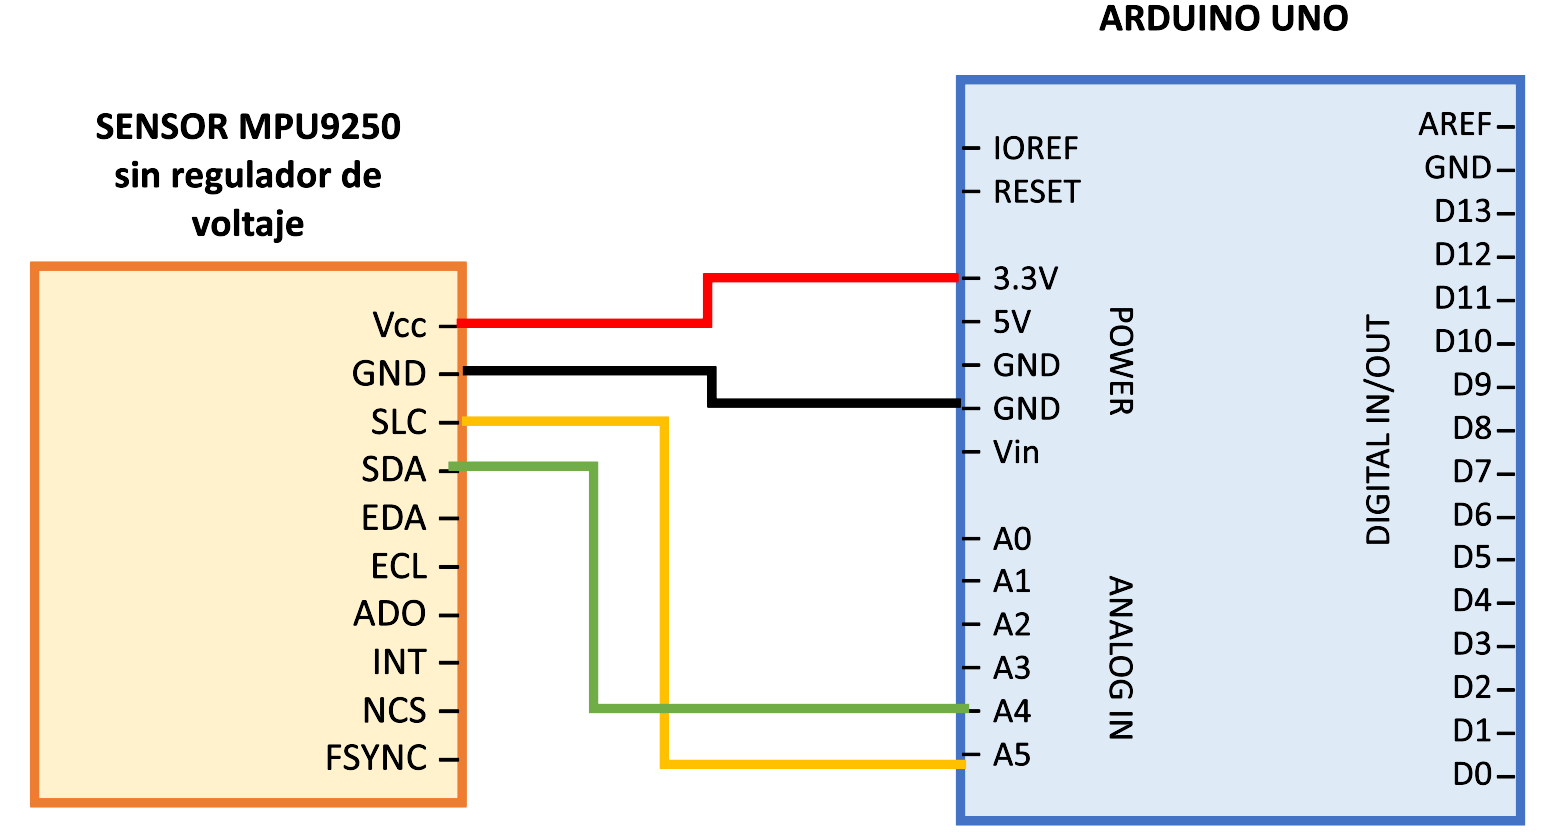
\includegraphics[width=0.5\textwidth]{img/MPU9250SinRegulador.png}
    \caption{Diagrama del módulo MPU9250 sin regulador de voltaje. Fuente Propia.}
    \label{fig:MPU9250} 
\end{figure}

\end{itemize}

\newpage


% ----------------------------------------------------
% Tabla de comparación de sensores
\begin{table}[h!]
\centering
\begin{tabular}{ |m{3.5cm}|m{8.5cm}|m{2cm}|  } 
\hline
\cellcolor[HTML]{B9E3F0}\textbf{Módulos} & \cellcolor[HTML]{B9E3F0}\textbf{Características} & \cellcolor[HTML]{B9E3F0}\textbf{Precio}\\

\hline
\cellcolor[HTML]{EFEFEF}\textbf{SCA60C}             & {Mide ángulos de 0-180º y necesita una tensión de entrada de 5V.}   & 15-25€\\
\hline
\cellcolor[HTML]{EFEFEF}\textbf{Galgas extensiométricas y módulos HX711}                & {Mide el peso que se ejerce sobre la galga, existen distintas galgas en función del peso a medir y necesita una tensión de entrada de 5V.} & 6-15€\\
\hline
\cellcolor[HTML]{EFEFEF}\textbf{ADXL345}                & {Tiene 3 DOF, mide las aceleraciones en los 3 ejes y necesita una tensión de entrada de 2-3.6V} & 3-10€\\
\hline
\cellcolor[HTML]{EFEFEF}\textbf{MPU6050}                & {Tiene 6 DOF, mide aceleraciones y ángulos de rotación en los 3 ejes y necesita una tensión de entrada de 2.4 a 3.6V.} & 5-15€\\
\hline
\cellcolor[HTML]{EFEFEF}\textbf{SW520D}                & {Detecta inclinaciones, es un sensor muy sencillo y actúa como un interruptor. Necesita una tensión de entrada de 5V.} & 0.3-5€\\
\hline
\cellcolor[HTML]{EFEFEF}\textbf{MPU9250}                & {Tiene 9 DOF, mide aceleraciones, ángulos y campos magnéticos en los 3 ejes. Elimina la deriva y necesita una tensión de entrada de 2.4 a 3.6V.} & 10-20€\\
\hline
\end{tabular}
\caption{Resumen y comparación de posibles sensores o módulos que se pueden emplear en el proyecto}
\end{table}


Una vez recopilados y comparados en la tabla anterior los posibles sensores que se podían emplear en el prototipo finalmente, se ha seleccionado el módulo SW520D para la realización de la primera versión del prototipo debido a su bajo coste, sencillez y disponibilidad. Para el segundo prototipo se decidió emplear el módulo MPU-6050, que es algo más complejo pero abre las posibilidades del prototipo, se ha seleccionado por sus características, sencillez de uso, precio y disponibilidad. Además, en un futuro, se podrían emplear otros módulos y también se podría ir estudiando y añadiendo otros componentes, cómo módulos Bluetooth o Baterías. Para encontrar más información de los prototipos consultar los anexos correspondientes.